% !TeX document-id = {e7fef4b9-afbc-4e81-94aa-c4847183d047}
% !BIB program = biber
\documentclass[10pt, times, conference, letterpaper]{IEEEtran}
\usepackage{nopageno}

%\usepackage[T1]{fontenc}
%\usepackage{amsfonts}
\usepackage{amsmath}
\let\openbox\relax
\usepackage{amsthm}
\usepackage[cmintegrals]{newtxmath}
\usepackage{bm}

\usepackage[dvipsnames]{xcolor}
\usepackage{graphicx}
\usepackage{tikz}
\usepackage{varwidth}
\usetikzlibrary{arrows.meta, calc, fit, positioning, shapes.misc}

\usepackage{etoolbox}
\usepackage[binary-units, per-mode=symbol]{siunitx}
\robustify\bfseries
\sisetup{detect-all, range-phrase=--, range-units=single, detect-weight=true,detect-inline-weight=math}

\makeatletter
\let\MYcaption\@makecaption
\makeatother

\usepackage[font=footnotesize]{subcaption}

\makeatletter
\let\@makecaption\MYcaption
\makeatother

\usepackage[basic]{complexity}
\usepackage[super,negative]{nth}

\usepackage[british]{babel}
\usepackage{csquotes}

\usepackage{booktabs}
\usepackage[
activate={true,nocompatibility},
final,
tracking=true,
kerning=true,spacing=true
]{microtype}
\microtypecontext{spacing=nonfrench}

%% Fix indent in new section...
\newcommand{\subparagraph}{}
\usepackage{titlesec}
\titlespacing*{\section}{0pt}{1.5ex}{0.7ex}
\titlespacing*{\subsection}{0pt}{1.5ex}{0.7ex}
\titlespacing*{\paragraph}{0pt}{1.5ex}{0.7ex}
\titlespacing*{\subsubsection}{0pt}{1.5ex}{0.7ex}
%\titleformat*{\filcenter\scshape}

\usepackage{enumitem}
\setlist[description]{leftmargin=8em,style=nextline}

%bib
\usepackage[style=ieee,maxnames=3,mincitenames=1,maxcitenames=2,maxbibnames=99,
mincrossrefs=99,minxrefs=99,
sortcites,
%backend=bibtex,
uniquelist=false]{biblatex}
\addbibresource{papers-off.bib}
\addbibresource{confs-off.bib}
\addbibresource{books-off.bib}
\addbibresource{rfc.bib}
\addbibresource{misc.bib}

%picky abt et al.
%\usepackage{xpatch}

%\xpatchbibmacro{name:andothers}{%
%	\bibstring{andothers}%
%}{%
%	\bibstring[\emph]{andothers}%
%}{}{}

% emph'd et al. for ieee style
\DefineBibliographyStrings{english}{%
	andothers = {\emph{et al}\adddot}
}
\DeclareFieldFormat[inproceedings]{url}{}
\DeclareFieldFormat[article]{url}{}
\DeclareFieldFormat[inproceedings]{doi}{}
\DeclareFieldFormat[article]{doi}{}
\DeclareFieldFormat[inproceedings]{editor}{}
\DeclareFieldFormat[proceedings]{editor}{}
\DeclareFieldFormat[article]{editor}{}

\usepackage{etoolbox}
\expandafter\patchcmd\csname citeauthor \endcsname
{\begingroup}{\begingroup\aftergroup\@}{}{}

% Thanks to http://codydunne.blogspot.com/2012/01/suppressing-bibtex-fields-for-specific.html
\AtEveryBibitem{% Clean up the bibtex rather than editing it
	\clearlist{address}
%	\clearfield{date}
%	\clearfield{eprint}
	\clearfield{isbn}
	\clearfield{issn}
	\clearlist{location}
%	\clearfield{month}
	\clearfield{series}
	
	\ifentrytype{book}{}{% Remove publisher and editor except for books
		\clearlist{publisher}
		\clearname{editor}
	}

	\ifentrytype{mics}{}{% Remove publisher and editor except for books
		\clearfield{url}
	}
}

%opening!

%\newcommand{\mytitle}{Improving Direct-Control Reinforcement Learning for Network Intrusion Prevention}
\newcommand{\mytitle}{Protocol-Agnostic DDoS Mitigation through Reinforcement Learning}

\usepackage{url}
\usepackage{hyperref}
\usepackage[nameinlink]{cleveref}
\newcommand{\crefrangeconjunction}{--}
\crefname{table}{table}{tables}

\hypersetup{
	colorlinks,
	citecolor=black,
	filecolor=black,
	linkcolor=black,
	urlcolor=black,
	pdftitle={\mytitle{}},
%	pdfauthor={Kyle A. Simpson, Simon Rogers, Dimitrios P. Pezaros}
	pdfauthor={Anonymous Giraffe, Anonymous Badger, Anonymous Ibex}
}
\newcommand*{\email}[1]{\href{mailto:#1}{\nolinkurl{#1}} } 

\usepackage{titling}
%\settowidth{\thanksmarkwidth}{*}
%\setlength{\thanksmargin}{-\thanksmarkwidth}
%
%%% Enable /thanks
%\IEEEoverridecommandlockouts
%\makeatletter
%\def\footnoterule{\relax%
%	\kern-5pt
%	\hbox to \columnwidth{\hfill\vrule width 0.5\columnwidth height 0.4pt\hfill}
%	\kern4.6pt}
%\makeatother

% make math easy
\newcommand{\acval}[3]{\ensuremath{\operatorname{\hat{q}}(#1, #2, #3)}}
\newcommand{\wvec}[1]{\ensuremath{\bm{w}_{#1}}}
\DeclareMathOperator*{\argmax}{argmax}

%thm environments
\newtheorem{thm}{Theorem}
\newtheorem{corr}{Corollary}[thm]

\newcommand{\fakepara}[1]{\noindent\textbf{#1:}}

\makeatletter\let\expandableinput\@@input\makeatother

\makeatletter
\DeclareRobustCommand{\rvdots}{%
	\vbox{
		\baselineskip4\p@\lineskiplimit\z@
		\kern-\p@
		\hbox{.}\hbox{.}\hbox{.}
}}
\makeatother

% Official colours!

\definecolor{uofguniversityblue}{rgb}{0, 0.219608, 0.396078}

\definecolor{uofgheather}{rgb}{0.356863, 0.32549, 0.490196}
\definecolor{uofgaquamarine}{rgb}{0.603922, 0.72549, 0.678431}
\definecolor{uofgslate}{rgb}{0.309804, 0.34902, 0.380392}
\definecolor{uofgrose}{rgb}{0.823529, 0.470588, 0.709804}
\definecolor{uofgmocha}{rgb}{0.709804, 0.564706, 0.47451}

\definecolor{uofglawn}{rgb}{0.517647, 0.741176, 0}
\definecolor{uofgcobalt}{rgb}{0, 0.615686, 0.92549}
\definecolor{uofgturquoise}{rgb}{0, 0.709804, 0.819608}
\definecolor{uofgsunshine}{rgb}{1.0, 0.862745, 0.211765}
\definecolor{uofgpumpkin}{rgb}{1.0, 0.72549, 0.282353}
\definecolor{uofgthistle}{rgb}{0.584314, 0.070588, 0.447059}
\definecolor{uofgpillarbox}{rgb}{0.701961, 0.047059, 0}
\definecolor{uofglavendar}{rgb}{0.356863, 0.301961, 0.580392}

\definecolor{uofgsandstone}{rgb}{0.321569, 0.278431, 0.231373}
\definecolor{uofgforest}{rgb}{0, 0.317647, 0.2}
\definecolor{uofgburgundy}{rgb}{0.490196, 0.133333, 0.223529}
\definecolor{uofgrust}{rgb}{0.603922, 0.227451, 0.023529}

\definecolor{inferno0}{rgb}{0.001462 0.000466 0.013866}
\definecolor{inferno64}{rgb}{0.341500 0.062325 0.429425}
\definecolor{inferno128}{rgb}{0.735683 0.215906 0.330245}
\definecolor{inferno192}{rgb}{0.978422 0.557937 0.034931}
\definecolor{inferno255}{rgb}{0.988362 0.998364 0.644924}

\colorlet{lowac}{inferno128}
\colorlet{midac}{inferno192}
\colorlet{highac}{inferno255}

%-------------------------------------%
%-------------------------------------%

\title{\mytitle{}}
\author{
%	Kyle~A.~Simpson\thanks{This work was supported by the Engineering and Physical Sciences Research Council [grant number EP/M508056/1].},
%	Kyle~A.~Simpson,
%	Simon~Rogers,
%	Dimitrios~P.~Pezaros,~\IEEEmembership{Senior~Member,~IEEE,},\\
%	School of Computing Science, University of Glasgow, Glasgow, G12 8RZ, UK\\
%	University of Glasgow, Glasgow, Scotland,\\
%	\email{k.simpson.1@research.gla.ac.uk}
Anonymous Giraffe,
Anonymous Badger,
Anonymous Ibex\\
Unnamed Department, Nowhere\\
\email{giraffe.a@unnamed.com}
}

% Remove date, leave no spacing.
\predate{}
\postdate{}
\date{}

\begin{document}

%% If needed, make urls typewritery
%\urlstyle{tt}

\maketitle

\begin{abstract}
DDoS attacks still cause significant harm to online services to this day.
Their detection is difficult, because like many cybersecurity problems they \emph{evolve}: normal and attack patterns shift due to new protocols and applications.
Such evolution makes it difficult to apply machine learning techniques and defences.

Reinforcement learning (RL) agents manage and monitor system health in an online manner.
Unsupervised, online learning is a key part of overcoming this detection problem.
We present the architecture of a system designed to host such RL agents in a typical network.
Furthermore, we introduce two agents which advance the state-of-the-art in using RL for DDoS mitigation.
Both of these act per flow, in a protocol-agnostic manner for any network topology.
This is supported by an in-depth investigation of feature suitability and empirical evaluation.

Our results show the existence of flow features with high predictive power for bulk TCP and VoIP traffic.
We show that the new agents offer a significant increase in throughput of legitimate TCP traffic for many choices of host density.
\end{abstract}

%\begin{IEEEkeywords}
%	Security services, distributed denial-of-service, software-defined networking, machine learning, reinforcement learning.
%\end{IEEEkeywords}

\section{Introduction}
%?? Redo intro to be more system focussed? Needs to be suitably different. Perhaps reduce focus on evolving, make it way more about "protocol-agnostic"...
%?? Just focus on DDoS, not anomaly detection writ-large

%?? DDoS attacks are bad...
Distributed Denial-of-Service (DDoS) attacks are a constant threat to online services.
Botnets like Mirai \cite{DBLP:conf/uss/AntonakakisABBB17} have been the primary driver of attacks against businesses like GitHub \cite{github-ddos-2018} (\SI{1.2}{\tera\bit\per\second}) and Dyn \cite{dyn-ddos-2016} (\SI{1.35}{\tera\bit\per\second}) in the past few years, bringing them offline by completely swamping the capacity of their servers and transit links.
%Memcrashed UDP amplification, 51000 factor for GitHub.
Existing DDoS defences typically rely on protocol behaviours and signatures, or upon proprietary middleboxes and traffic scrubbing services.
%?? What happens when we roll out new protocols? Particularly those which focus on obfuscation? Behaviours become completely opaque, and ossification works against us.
These defence strategies are effective around their time of invention, but rely upon network ossification to remain relevant.

However, the internet is always in flux.
The constant deployment of new services and protocols means that traffic is \emph{non-stationary} and evolving.
This ranges from subtle variation, such as new TCP congestion control algorithms \cite{rfc8312}, to the rapid rollout \cite{DBLP:conf/pam/RuthPDH18} of future protocols like QUIC \cite{DBLP:conf/sigcomm/LangleyRWVKZYKS17}.
%?? What happens when we roll out new protocols? Particularly those which focus on obfuscation? Behaviours become completely opaque, and ossification works against us.
Reliance on a fixed network is at odds with reality, when QUIC causes a large proportion of (traditionally) constant bitrate UDP traffic to become congestion-aware.
Behaviours and signatures become harder still to extract if the main purpose of a protocol is obfuscation (again, as in QUIC).
%?? Also attacks evolve.
DDoS attacks themselves also evolve in both short and long timescales (i.e., a sequence of attack strategies vs.\@ unseen attacks) \cite{DBLP:conf/spw/KangGS16}.
Thus, we must look at defence models which can identify characteristics and behaviours of DDoS traffic \emph{automatically}.

%Network anomaly detection and intrusion detection/prevention are continually evolving problems, compounded by the partial, non-\emph{independent and identically distributed} (IID) view of data at each point in the network.
%Attacks and anomalous behaviours evolve, becoming more sophisticated or employing new vectors to harm a network or system's confidentiality, integrity, and availability without being detected \cite{DBLP:journals/comsur/BhuyanBK14}.
%These attacks and anomalies have measurable consequences and symptoms which allow a skilled analyst to infer new signatures for detection by misuse-based classifiers, but unseen attacks may only be defended against after-the-fact.
%This issue is inherent to \emph{misuse-} or \emph{signature-based} intrusion detectors, and it has been long-hoped that \emph{anomaly-based} detectors would surpass this by making effective use of statistical measures \cite{DBLP:journals/comsur/BhuyanBK14}.

%?? Then talk about ML. And its costs, say that its ADS/IDS weaknesses extend to DDoS prevention.
While \emph{machine learning} (ML) approaches seem suitable for this problem, there is a distinct lack of real-world deployments in the broader field of intrusion detection/prevention.
\Textcite{DBLP:conf/sp/SommerP10} posit that this stems from greater risks than other ML tasks: the high cost of errors, low tolerance for false positives; a lack of recent, high-quality training data; and traffic diversity and evolution.
It is immediately clear that these challenges also apply to DDoS prevention.
Learning is made harder still by the challenges encountered when learning from unlabelled or partial data.
%DDoS prevention exhibits many of these issues.
%?? Then Bam! Introduce RL.

\emph{Reinforcement learning} (RL) offers another perspective.
%?? Unclear explanation of RL here?
RL agents follow a \emph{policy} to interact with or control a system, while at the same time using observed performance to improve this policy online.
An agent then adaptively reacts to threats by acting as a feedback loop for network optimisation---this allows us to overcome some of these difficulties by monitoring the consequences of each action in real-time.
We aim to prevent volume-based DDoS attacks with the aid of RL-based techniques, while bringing to light the flexibility of these techniques in the security domain.
%Whether it takes direct control of the network, or is used indirectly to optimise a key part of another system, more powerful `deep' RL techniques (and well-founded action spaces) aren't yet well explored for network IDS/IPS.
%These range from more modern training algorithms \cite{DBLP:journals/corr/SchulmanWDRK17, DBLP:conf/icml/SchulmanLAJM15}, to evolutionary strategies \cite{DBLP:journals/corr/SalimansHCS17, DBLP:journals/corr/abs-1802-08842}, hierarchical action composition \cite{DBLP:journals/corr/abs-1710-09767}, and competitive multi-agent learning \cite{DBLP:journals/corr/abs-1710-03748}.
%?? This raises the question: how do we do this effectively? Agents need state and reward info, which can be a lot of data transfer. THis gets worse (hint: we have the answer...)
This introduces a new set of problems: what effective state/action spaces should look like, how state and reward information should be efficiently propagated, and how this can be achieved on commodity hardware.

%?? Discuss the most important conclusions before the outline.
We find that the existing RL work for this task fails to account for congestion-aware traffic (i.e., TCP, QUIC) and environments with high host density at ingress points.
To remedy this, our agents make throttling decisions per-source, and show how an action model built on domain-specific knowledge can increase performance.
This requires additional engineering: updating RL agents from multiple traces per timestep, smart work scheduling, and an architecture featuring (but minimising) the use of software-defined networks (SDN).
%In tandem with the development and evaluation of an effective state space and model, we provide the design of a second model inspired by past work on algorithmic DDoS prevention, as an example of the integration of domain-specific knowledge.
This improves substantially upon the state-of-the-art when acting upon most internet traffic (i.e., congestion-aware protocols), and we show that the use of domain knowledge achieves excellent performance at high host density.
Crucially, the models are protocol- and content-agnostic to offer future-proofing against the rollout of future protocols.
%?? Also algorithmic enhancements such as multiple actions per timestep, 
%?? PROTOCOL-AGNOSTIC -- HOW WILL THESE THINGS COPE WITH QUIC ET AL.?!?!
Briefly, this paper contributes:
\begin{itemize}
%	\item A DDoS mitigation system based on direct-control reinforcement learning, designed for deployment in real-world software-defined networks (\cref{sec:environment-and-rl-algorithm,sec:acting-on-individual-sources}).
%	\item Important weaknesses and flaws in the past design and evaluation of similar techniques \cite{DBLP:journals/eaai/MalialisK15}. We offer a deconstruction and empirical study on their formulation, flaws, and risk factors concerning different traffic distributions---in addition, we demonstrate modifications enabling deployment in real-world software-defined networks (\cref{sec:performance-in-an-emulated-environment}).
	\item Two source-level granularity models for RL-driven DDoS prevention (\emph{Instant} and \emph{Guarded} action models) and suitable features (\cref{sec:ddos-mitigation-with-per-flow-reinforcement-learning}).
	\item A description of the system architecture which supports the real-world deployment of such agents (\cref{sec:system-architecture}).
%	\item An investigation of suitable features for this task (\cref{sec:rethinking-the-state-space}).
	\item Reactive simulations of HTTP and VoIP web-server traffic (\cref{sec:a-new-normal}).
	\item A performance comparison of different RL algorithms within these agents, and against the state-of-the-art in RL-based DDoS mitigation (\cref{sec:the-results-of-doing-so}).
%	\item An empirical evaluation of our new models against the state-of-the-art in RL-based DDoS mitigation (\cref{sec:the-results-of-doing-so}).
\end{itemize}

\section{Background}
%?? Introduce RL, related definitions etc.

\subsection{Distributed Denial of Service}
%?? DDoS attack variants (leading into characteristics, supporting features). Amplification (UDP \cite{DBLP:conf/ndss/Rossow14}, TCP \cite{DBLP:conf/uss/KuhrerHRH14}), Transit-link (Crossfire \cite{DBLP:conf/sp/KangLG13}, Coremelt \cite{DBLP:conf/esorics/StuderP09}). Mirai botnet's involvement \cite{DBLP:conf/uss/AntonakakisABBB17}.

%?? Explain amplification attack, maybe transit-link?

\emph{Distributed denial of service} (DDoS) attacks are concentrated efforts by many hosts to reduce the availability of a service, to inflict financial harm or as an act of vandalism.
Attackers achieve this by exploiting system or application behaviour in \emph{semantic attacks} (e.g., \emph{SYN flooding attacks}), or by overwhelming their target through requests or traffic (\emph{volume-based attacks}) \cite{DBLP:conf/imc/JonkerKKRSD17}.
Hosts often participate unwillingly, typically having been recruited into a \emph{botnet} by malware infection to be orchestrated from elsewhere \cite{DBLP:conf/uss/AntonakakisABBB17}.

Volume-based attacks are the most relevant to our work, with two varieties being especially prevalent.
\emph{Amplification attacks} exploit services who send large replies in response to small requests, with UDP-based services like DNS and NTP seeing most abuse \cite{DBLP:conf/ndss/Rossow14, DBLP:conf/uss/KuhrerHRH14}.
Malicious hosts send many small requests, spoofed using the victim's address, causing many large replies to be sent to the intended target---increasing a botnet's throughput while keeping participants anonymous.
\emph{Transit-link/link-flooding attacks} have been the subject of recent attention, wherein malicious traffic is forwarded across core links needed to reach a target (but not to the target itself) \cite{DBLP:conf/sp/KangLG13, DBLP:conf/esorics/StuderP09}.

\subsection{Reinforcement Learning}\label{sec:reinforcement-learning}
\emph{Reinforcement learning} (RL) is a variant of machine learning concerned with training an agent to choose an optimal sequence of actions for a given task \cite{RL2E}.
We assume at any point in time $t$, an agent knows which \emph{state} it is in ($S_t \in \mathcal{S}$), the set of \emph{actions} which are available to it ($\operatorname{A}(S_t) \subseteq \mathcal{A}$) and numeric \emph{reward} obtained from the last action chosen ($R_t \in \mathbb{R}, A_{t-1} \in \operatorname{A}(S_{t-1})$).
This model of system interaction is a \emph{Markov Decision Process} (MDP), where agents aim to maximise the \emph{expected reward} received.
RL methods combine this information with a current \emph{policy} $\pi$ to determine which action should be taken.
The policy is refined as more decisions and rewards become available, learning online.
In practice, this means that agents are able to automatically adapt to evolving problems without operator intervention or a new training corpus.

%?? Include some details of function approximation in the formalisation? I.e. tile coding, stability and convergence guarantees...
We focus on methods based on action value estimates from the current state: let $\operatorname{q}(s, a) \in \mathbb{R}$ denote the estimate of action $a$'s value if it were to be taken in state $s$.
%?? Revisit the maths here, d, dim A, s...
To cope with a continuous state and/or action space, one technique to obtain this value is to employ linear function approximation backed by \emph{tile coding} \cite[pp.\ \numrange{217}{221}]{RL2E}.

\begin{figure}
	\centering
	\begin{subfigure}{0.4\linewidth}
		\resizebox{\linewidth}{!}{
		\begin{tikzpicture}
		\node at (0,0.3){$s = \begin{pmatrix}
			0.7 \\
			0.3
			\end{pmatrix}$};
		\node at (0,-1) {$\bm{x}(s,\cdot) = \begin{Bmatrix}
			T_{1,9}, \\
			T_{2,5}, \\
			T_{\mathit{bias}}
			\end{Bmatrix}$};
		
		\node at (2.5,-0.5) {
			\begin{tikzpicture}
			\draw[step=0.5cm,color=uofgcobalt,opacity=0.7,shift={(0,0)},label=above:{Tiling 0}] (-0.5,-0.5) grid (1,1);
			\fill[uofgcobalt,opacity=0.5] (0.5,-0.5) rectangle (1,0);
			\node[color=uofgcobalt] at (0,1.1) {\footnotesize Tiling 1};
			
			\draw[step=0.5cm,color=uofgpumpkin,opacity=0.9,shift={(0.25,-0.25)},label=above:{Tiling 1}] (-0.5,-0.5) grid (1,1);
			\fill[uofgpumpkin,opacity=0.5,shift={(0.25,-0.25)}] (0,0) rectangle (0.5,0.5);
			\node[color=uofgpumpkin!50!uofgrust] at (0.25,-0.95) {\footnotesize Tiling 2};
			
			\node[circle, black, draw,
			fill, radius=0.5pt, inner sep=0pt,minimum size=1.5pt, label=above:{$s$}] at (0.625,-0.125) {};
%			\filldraw (0.625,-0.125) circle[radius=1.5pt,label=above:{$s$}];

			\draw[->] (-0.25,-0.5)--(-0.25,0.85);
			\draw[->] (-0.25,-0.5)--(1.1,-0.5);
			
			\node at (1,-0.7) {\footnotesize 1};
			\node at (-0.4,0.75) {\footnotesize 1};
			\node at (-0.35,-0.6) {\footnotesize 0};
			\end{tikzpicture}
		};
		
		\end{tikzpicture}
		}
		\caption{Tile Coding\label{fig:tilecode-code}}
	\end{subfigure}%
	\begin{subfigure}{0.4\linewidth}
		\resizebox{\linewidth}{!}{
		\begin{tikzpicture}
		% Top half
		\def\topacs{
			{-0.3,-0.5,-0.1,0.8},
			{0.1,0.1,-0.2,0.3},
			{0.3,0.4,0.2,-0.4}%
		}
	
		\foreach \line [count=\y] in \topacs {
			\foreach \pix [count=\x] in \line {
				\ifthenelse{\lengthtest{\pix pt < 0 pt}}{
					\pgfmathtruncatemacro\lambda{(\pix+1)*100}
					\draw[shift={(-0.7,0)},fill=midac!\lambda!lowac] (0.7*\x,-0.35*\y) rectangle +(0.7,0.35);
				}{
					\pgfmathtruncatemacro\lambda{\pix*100}
					\draw[shift={(-0.7,0)},fill=highac!\lambda!midac] (0.7*\x,-0.35*\y) rectangle +(0.7,0.35);
				}
				\node[shift={(-0.35,0.175)}] at (0.7*\x,-0.35*\y) {\footnotesize \pix};
			}
		}
	
		\draw[xstep=0.7cm,ystep=0.35cm,shift={(0,0)}] (0,-1.06) grid (2.8,0);
		\node[label=left:{$T_{1,9}$},shift={(0,-0.125)}] at (0,0) {}; 
		\node[label=left:{$T_{2,5}$},shift={(0,-0.125)}] at (0,-0.375) {}; 
		\node[label=left:{$T_{\mathit{bias}}$},shift={(0,-0.125)}] at (0,-0.75) {};
		
		% bottom half
		\def\botacs{
			{0.1,0.0,-0.1,0.7}%
		}
	
		\foreach \line [count=\y] in \botacs {
			\foreach \pix [count=\x] in \line {
				\ifthenelse{\lengthtest{\pix pt < 0 pt}}{
					\pgfmathtruncatemacro\lambda{(\pix+1)*100}
					\draw[shift={(-0.7,-1.275)},fill=midac!\lambda!lowac] (0.7*\x,-0.35*\y) rectangle +(0.7,0.35);
				}{
					\pgfmathtruncatemacro\lambda{\pix*100}
					\draw[shift={(-0.7,-1.275)},fill=highac!\lambda!midac] (0.7*\x,-0.35*\y) rectangle +(0.7,0.35);
				}
				\node[shift={(-0.35,-1.1)}] at (0.7*\x,-0.35*\y) {\footnotesize \pix};
			}
		}
	
		\draw[xstep=0.7cm,ystep=0.35cm,shift={(0,-1.275)}] (0,-0.35) grid (2.8,0);
		\node[label=left:{$\mathit{Total}$},shift={(0,-0.175)}] at (0,-1.275) {};
		
		\draw [->] (2.45, -1.9) -- (2.45, -1.65);
		\end{tikzpicture}
		}
		\caption{\centering Value Estimation and Action Selection\label{fig:tilecode-select}}
	\end{subfigure}
	
	\caption{
		An example of tile coding for 2-dimensional state and 4 actions, using 2 tilings, 3 tiles per dimension, and a bias tile.
		\vspace{-1em}
		\label{fig:tilecode}
	}
\end{figure}

Tile coding is a form of feature representation which converts a state-action pair into a sparse boolean feature vector $\operatorname{\mathbf{x}}(s, a)$ by subdividing a $d$-dimensional subset of the space into a number of overlapping grids.
Each tile corresponds to an entry of $\operatorname{\mathbf{x}}(s, a)$ which is set to 1 if the state-action pair lies within it.
\Cref{fig:tilecode-code} demonstrates the process for a 2-dimensional state space, and that the numbers of tilings and tiles per dimension control feature resolution and generalisation.
We may then approximate an action's value with respect to a policy parameter vector $\wvec{}$, defining some $\acval{s}{a}{\wvec{}} \approx \operatorname{q}(s, a)$:
\begin{equation}
%	\begin{gather}
\acval{s}{a}{\wvec{}} = \wvec{}^{\top} \operatorname{\mathbf{x}}(s, a)
%	\end{gather}
\label{eqn:lin-approx}
\end{equation}
As each component of $\wvec{}$ is the value estimate of the corresponding tile, learning an effective policy is equivalent to learning $\wvec{}$.
Given a learning rate $\alpha \in \mathbb{R}$ and initialising $\wvec{0}=\bm{0}$, we may continually update $\wvec{t}$ using the \emph{1-step semi-gradient Sarsa} algorithm \cite[pp.\ \numrange{243}{244}]{RL2E}:
\begin{subequations}
	\begin{gather}
	\delta_t = R_{t+1} + \gamma \acval{S_{t+1}}{A_{t+1}}{\wvec{t}} - \acval{S_t}{A_t}{\wvec{t}},\\
	\bm{w}_{t+1} = \bm{w}_{t} + \alpha \delta_t \nabla{\acval{S_t}{A_t}{\wvec{t}}},
	\end{gather}%
	\label{eqn:sg-sarsa}%
	where $\delta_t$ is known as the \emph{temporal-difference} (TD) error, the \emph{discount factor} $\gamma \in [0,1)$ determines how crucial future rewards are, and the vector gradient $\nabla$ is taken with respect to $\wvec{}$.
\end{subequations}

Computing the approximate value of every action available in the current state forms the basis of a policy.
To encourage early exploration, actions with maximal value can be chosen each time except when taking random actions with probability $\epsilon$---an \emph{$\epsilon$-greedy policy}).
Each action $a \in \operatorname{A}(s)$ has probability $\pi(a|s,\wvec{})$ of being chosen:
\begin{equation}
	\pi(a|s,\wvec{}) =
	\begin{cases}
	1 - \epsilon + \epsilon/{|}{\operatorname{A}(s)}{|} & \text{if $a = \operatorname*{argmax}\limits_{a'} \acval{s}{a'}{\wvec{}}$} \\
	\epsilon/{|}{\operatorname{A}(s)}{|} & \text{otherwise}
	\end{cases}
\end{equation}
\Cref{fig:tilecode-select} shows how the value of each action is computed (and which action would be chosen by a greedy policy).

This combination of algorithm and coding strategy is well-optimised, if actions are discrete.
A particularly efficient (vectorised) implementation is described by \textcite{RL2E}---briefly, we need only perform $n_{\mathit{tilings}} + 2$ additions and \num{2} multiplications per model update and constant action computation cost ($\mathcal{O}(n_{\mathit{tilings}})$).

\subsection{Motivation}\label{sec:motivation}
%?? What makes RL a suitable method for network anomaly detection, what features are most relevant?
%?? Point I was thinking of: feedback-loop-like model allows monitoring \emph{after} an action is taken to (in theory) allow forgiveness of mistakenly punished flows. This does hinge on taking a flow-by-flow look at the state space, but if we can combine knowledge of current state (duh!), the last action taken (i.e. an indicator of our previous assessment [such as high pdrop $\implies$ bad]) then perhaps a flow which falls off identically to a legit flow can be rescued.
There are concrete reasons to use RL methods in this domain, beyond handling non-stationarity.
Misclassification is a serious problem, introducing \emph{collateral damage} in a DDoS prevention system.
RL's feedback-loop model lets us monitor flows \emph{after} an action is taken to perhaps allow forgiveness of mistakenly punished flows.
This relies upon a flow-by-flow view of the state space, but knowledge of the current state and last applied action detect whether punished flows fall off identically to legitimate flows.

%Which features might be best suited to this problem?
%?? Relevant features: aggregate network state (load at various points [this has been done, of course]), flow-specific measurements (upload/download ratio when bandwidth above threshold \cite{DBLP:conf/ndss/Rossow14}, packet inter-arrival times, etc.)
Other studies suggest that there are particularly useful features which make the task of online DDoS flow identification feasible.
Link loads observed at various locations suggest the overall health of a network \cite{DBLP:journals/eaai/MalialisK15}, and the ratio of correspondence between pair flows can suggest illegitimacy \cite{DBLP:conf/ndss/Rossow14}.
Volume-based statistics (counts, counts per duration, average packet sizes) have seen use in $k$-nearest neighbours classifiers trained to detect DDoS attacks \cite{DBLP:conf/dsn/LeeKSPY17}.
Most importantly, there is evidence showing that bandwidth expansion may cause behavioural changes which differ between benign and attack traffic \cite{DBLP:conf/ndss/KangGS16}.

\section{DDoS Mitigation with Per-flow Reinforcement Learning}\label{sec:ddos-mitigation-with-per-flow-reinforcement-learning}
We hypothesise that per-flow agent designs will offer better accuracy than current RL-based agents for DDoS mitigation.
We describe and justify our approach and algorithmic improvements, presenting two action models, one of which draws on domain knowledge introduced by SPIFFY \cite{DBLP:conf/ndss/KangGS16}.

\subsection{System Design and Assumptions}
Agents are deployed in a network with a set of \emph{ingress/egress points} from its domain of control through which traffic can flow, and a set of protected \emph{destination nodes}.
These destination nodes may be services, servers, or in the case of Autonomous Systems (ASes) and transit networks, egress points leading to other networks.
Agents are co-located with each egress switch, and control the proportion of upstream packets from each external host to discard.
Each destination node $s$ has a maximum capacity, $U_s$.

\subsection{Algorithm}
To make decisions and learn cheaply with low latency, we use \emph{semi-gradient Sarsa with tile coding} (\cref{eqn:sg-sarsa}).
Exploration is introduced by making use of $\epsilon$-greedy action selection, linearly annealing $\epsilon$ to 0 over time.
Each agent has its own internal parameter vector $\wvec{}$.

While classical RL methods likely have lower accuracy than more complex approximators like neural networks, there are reasons to favour them; faster decisions, lower energy usage, reduced model complexity (and training time), and the availability of compatible hardware.
This aligns with the goal of quick online learning and fast adaptation to traffic changes, without introducing dedicated tensor processing hardware.
Approaches like this also have simpler decision boundaries, reducing the risks of overfitting and unexpected behaviour, while possibly aiding in interpreting anomalous action choices.

\subsubsection{Action rate}
The algorithm is adapted to prioritise rapid response to changes in network state and to visit as many state-to-state transitions as possible to learn quickly.
Agents thus make many decisions per timestep.
We update $\wvec{}$ using each decision made and the reward signal from the relevant destination.
As exploration still occurs for each action, $\epsilon$ must be reduced multiple notches every timestep.
In turn, we increase the annealing window for $\epsilon$ by a factor of \num{2.67} so as to preserve exploration over time, by accounting for the greater volume of decisions being made.

\subsubsection{Per-tile updates}
To adjust the value of each activated tile with a different magnitude and direction, we compute a different temporal difference value \emph{for each tiling}.
This corrects tiles which contribute too much or too little value without disturbing estimates which are almost correct.
While we make use of all tiles' action value estimates when making decisions, each tiling is updated using only its own contribution, allowing us to increase $\alpha$ without divergence.
Compared to the standard algorithm, effective policies are reached sooner.

\subsubsection{Decision narrowings}
When learning a high-dimensional tile-coding, assignment of credit for each decision is difficult because all tiles have identical gradient---i.e., assigning credit to the \emph{features} which drove each decision is difficult.
To combat this, with probability $\epsilon$ an agent will mark a flow as being governed by a subset of the state space for the next five decisions.
Each agent chooses actions for that flow using \emph{one element of local state}, the global state, and the bias tile---we include the latter two to strike a balance between and accuracy and correct credit assignment.

\subsection{Feature Space}\label{sec:feature-space}

\begin{figure}
	\centering
	\resizebox{0.65\linewidth}{!}{
		\begin{tikzpicture}[
		texts/.style = {text=black},
		labeltexts/.style = {text=gray},
		treeline/.style = {draw=uofgburgundy},
		treenode/.style = {texts, circle, centered, fill=white, treeline},
		load/.style = {fill=uofgcobalt},
		loadline/.style = {draw=uofgcobalt, line width=0.75mm},
		loadhide/.style = {fill=uofgcobalt!40!white},
		external/.style = {fill=uofgrust},
		externalhide/.style = {fill=uofgrust!40!white},
		hideline/.style = {draw=uofgsandstone!40!white},
		hidenode/.style = {treenode, hideline},
		grow'=right
		]
		\node [treenode, loadhide, label={[texts]above:Agent 1}] (mainagent) {};
		\node [treenode, loadhide, right = of mainagent] (inner0) {};
		\node [treenode, loadhide, above right = 0.2cm and 1cm of inner0] (inner1) {};
		\node [hidenode, below right = 0.2cm and 1cm of inner0] (inner2) {};
		\node [treenode, loadhide, below right = 0.2cm and 1cm of inner1] (inner3) {};
		\node [treenode, loadhide, right = of inner3] (inner4) {};
		\node [treenode, loadhide, above right = 0.2cm and 1cm of inner4, label={[texts]above:$s_0$}] (s0) {};
		\node [hidenode, below right = 0.2cm and 1cm of inner4, label={[labeltexts]above:$s_1$}] (s1) {};
		
		\node [hidenode, above left = 0.2cm and 0.5cm of inner1, label={[labeltexts]above:Agent 2}] (agent2) {};
		\node [hidenode, below left = 0.2cm and 0.5cm of inner2, label={[labeltexts]below:Agent 3}] (agent3) {};
		
		\draw[hideline, -] ($ (mainagent) + (-1,0) $) -- (mainagent);
		\draw[hideline, -] ($ (agent2) + (-1,0) $) -- (agent2);
		\draw[hideline, -] ($ (agent3) + (-1,0) $) -- (agent3);
		\draw[hideline, -] (inner1) -- (agent2);
		\draw[hideline, -] (inner2) -- (agent3);
		
		\draw[loadline, -] (mainagent) -- (inner0);
		\draw[loadline, -] (inner0) -- (inner1);
		\draw[hideline, -] (inner0) -- (inner2);
		\draw[-] (inner1) -- (inner3);
		\draw[hideline, -] (inner2) -- (inner3);
		\draw[loadline, -] (inner3) -- (inner4);
		\draw[loadline, -] (inner4) -- node [texts, above] {$U_{s_0}$} (s0) ;
		\draw[hideline, -] (inner4) -- node [labeltexts, below] {$U_{s_1}$} (s1);
		
		\end{tikzpicture}
	}
	\caption{
		Global state selection for a flow between an external host and server $s_0$ which passes over Agent 1.
		Nodes in the path taken are filled in blue, and link load measurements which are used for decisions are indicated with a thick blue line.
		\vspace{-1em}
		\label{fig:global-state-path}
	}
\end{figure}

Our state space combines global state (network load) with per-flow measurements.
Each is tile-coded with 8 tilings and 6 tiles per dimension, using the windows described in \cref{tab:codings}.
Features are tiled separately, with the exception of packet in/out count (per-window and total), mean in/out packet size, and $\Delta$ in/out rate, which are combined with the last action taken.

%?? How is global state acquired? See \cref{fig:global-state-path}. Why take paths in the way that we do? Mention deterministic ECMP routing etc...
Global state is a vector of load values in $\mathbb{R}^4$ (\si{\mega\bit\per\second}): the bandwidth measurements regularly received from monitors in the environment.
For any flow, an agent computes the path it would take through the network.
The incoming load along the first hop, last hop, and tertiles of the path are then tile-coded together.
In the event that this path is shorter than 4 hops, we duplicate (in order of preference) a middle hop or the last hop.
\Cref{fig:global-state-path} illustrates the process.
Global state built in this way is compatible with multipath, multi-destination networks, offering support for diverse deployment environments from endpoint servers up to transit ASes.
Computing a flow's path is not computationally expensive: multipath routing is fast since typical ECMP routing algorithms simply hash a packet's 5-tuple and are deterministic to provide consistent quality-of-service.

%?? Path computation fast and efficient due to deterministic routing based on hashes (ECMP)
%?? Works for any arbitrary topology, even 

\Cref{fig:udp-feature-plots} shows the effectiveness of per-flow features for UDP (resp.\ \cref{fig:tcp-cap-feature-plots} for TCP), on a single-destination topology (\cref{sec:single-dest}) with $n=2$ hosts per egress point averaged over 10 episodes.
The plots demonstrate that different protocols and traffic classes are best defended by different features---every feature presented has value in a complete model.
Packet-level and per-window statistics are at their best when combined with the last action for both UDP-like and TCP-like traffic (omitted).
All features converge to their highest-observed performance within around \num{4000} timesteps.
In general, some of the most effective features are global state, mean IAT, mean inbound packet size and $\Delta$ rates.
The exclusion of features such as source/destination ports or protocol numbers is a deliberate choice.
If \emph{QUIC} (or a similar protocol) were to become ubiquitous, then these fields would have no correlation with the class of traffic a flow contains.

\subsection{Reward Function}

%?? Say ``we take $R_G$ from M and K''.
%
%?? Reward at each destination.

\newcommand{\arrload}[2]{\operatorname{load}^{#2}_{t}(#1)}
\newcommand{\uload}[1]{\arrload{#1}{\uparrow}}
\newcommand{\dload}[1]{\arrload{#1}{\downarrow}}
\newcommand{\bload}[1]{\arrload{#1}{\updownarrow}}
\newcommand{\cond}[2]{\operatorname{c}_{#1,t}#2}
%\fakepara{Reward function directionality}
%The reward functions, as defined, do not take traffic direction into account.
%We redefine these to identify overload states using both upstream and downstream loads, while allowing customisation of which direction is chosen for protection.
We denote the upstream, downstream and combined loads at a node $s$ as $\uload{s}, \dload{s}, \bload{s}$ respectively.
Each destination node $s$ generates a reward signal, $R_{s,t}$, at every timestep $t$.
Assuming each destination has access to some classification function $g(\cdot)$ which estimates the volume of legitimate traffic received, and expects to receive $\mathit{traffic}_s$, we may compute the reward:
\begin{subequations}
%	\vspace{-0.5cm}
	\newcommand{\load}[1]{\operatorname{load}_{t}(#1)}
	\begin{gather}
	\cond{s} = [\max(\uload{s}, \dload{s}) > U_s],\\
	R_{s,t} = (1 - \cond{s}) \frac{g(\arrload{s}{-})}{\mathit{traffic}_s} - \cond{s},\label{eqn:reward-rtx}
	\end{gather}
	replacing $\arrload{s}{-}$ in \cref{eqn:reward} with whichever directional load is prioritised according to the traffic characteristics of the deployment environment, where $\cond{s}$ represents the ``overloaded'' condition at destination $s$.\label{eqn:reward}
\end{subequations}
We choose $\uload{\cdot}$ for our UDP-based models and $\dload{\cdot}$ for HTTP, and suggest $\bload{\cdot}$ for general deployment or heterogeneous traffic.
These choices reflect where the bulk of transmitted bytes in each traffic model are observed (or the lack of this knowledge).

While our use and definition of $g(\cdot)$ appears nebulous, there are many ways to infer this quantity in practice.
End-host servers may make use of canary flows or active measurement schemes, and can employ quality-of-experience metrics in the case of VoIP services such as lost packets, reorderings, and jitter.
ASes and transit networks may make use of reports received from downstream networks, i.e. over the \emph{DDoS Open Threat Signalling} (DOTS) protocol \cite{ietf-dots-use-cases-17}.
We leave the use of such data as future work.
Even without online rewards, a well-trained agent needs only to follow the greedy policy it has learned from offline (simulated) training.

If a network is believed to be vulnerable to indirect attacks, such as link-flooding attacks, we may use the following reward:
\begin{equation}
	R_{s,t}^{\mathit{Cross}}(\beta) = \beta R_{s,t} + (1 - \beta) \min{\{R_{s',t} | s' \ne s\}} \label{eqn:lfa-reward}
\end{equation}
where the collaboration parameter $\beta \in [0,1]$ models the expected degree of interference between flows, and $s, s'$ are protected destination nodes in the network.
The key insight underpinning LFAs is that flows can affect a target \emph{without communicating with that target}.
$\beta$ then acts as a tunable parameter which can incentivise agents to remove flows which harm overall system health, by including the performance of the worst-performing destination.
However, we do not examine such attacks (and the effectiveness of $R_{s,t}^{\mathit{Cross}}$) at present.

\subsection{Action Space}
When monitoring a flow, an agent uses its state vector to decide which portion of its \emph{inbound} traffic should be dropped.
%?? Why pdrop? Allows for discrete action space, don't have to account for buckets/fairness/burstiness.
We choose to drop packets (rather than impose traffic limits) to have a discrete action space without prior knowledge of traffic characteristics.
Furthermore, we need not consider burstiness, fairness and parameters such as bucket sizes which could require tuning.
We offer two models, which differ only on how to choose $p$.
The intuition behind these designs is that an agent may directly choose the level of packet drop at the expense of a larger action space (\emph{Instant control}), or that we may reduce the action set (and learn a policy within fewer actions) by making use of domain knowledge (\emph{Guarded control}).

\subsubsection{Instant control}
Each agent directly chooses $p \in \left\{ 0.0, 0.1, \ldots, 0.9 \right\}$.
These choices ensure that the rate reduction imposed on a source IP may never be permanent or irreversible.
Since this model requires no forward planning, we found it best to set the discount factor $\gamma=0$ (making agents purely opportunistic/myopic).

\subsubsection{Guarded control}
\Textcite{DBLP:conf/ndss/KangGS16} suggest that bot attack flows cannot scale up to match an increase in available bandwidth.
We apply their observations, constraining how an agent treats each flow via simple finite state automata: restricting $p \in \left\{ 0.00, 0.05, 0.25, 0.50, 1.0 \right\}$.
The action set is then simply to \emph{maintain}, \emph{increase}, or \emph{decrease} $p$ for a flow in single steps.

We choose these potential values for $p$ to add complete filtering to a steady progression of rate-limits (\SI{25}{\percent} increments for UDP traffic).
The outlier, $p=0.05$, corresponds to roughly a \SI{50}{\percent} rate reduction for TCP flows in our test topology.
This uneven spread of choices for $p$ allows light and heavy rate reduction to be applied to both congestion-aware and congestion-unaware traffic as required.
As each agent now requires the capability to plan ahead, we require a discount factor $\gamma \ne 0$, allowing the value of future states to influence state-action value updates.
We found the setting $\gamma = 0.8$ to be the most effective choice during exploratory testing.

To enable temporary bandwidth expansion in all deployments, every flow is initially placed under light packet drop ($p=0.05$), chosen due to TCP's higher prevalence.
An agent must now choose to punish a flow multiple times in succession to block it, reducing variance while allowing an agent to see how a host reacts to controlled conditions.
While beneficial for legitimate flows who behave similarly to attack traffic, this introduces a lag of an extra two actions in blocking illegitimate flows.

\subsubsection{Risks}
Our mode of action means that each agent carries a risk of introducing collateral damage into the network.
This is particularly severe when handling TCP traffic: the Mathis equation \cite{DBLP:journals/ccr/MathisSMO97} states that TCP bandwidth is proportional to $1/\sqrt{p}$ (noting that $p\ne0$ in any real network) while constant bitrate (CBR) UDP traffic is proportional to $1 - p$.
This weakness remains in modern flavours of TCP---TCP Cubic has bandwidth proportional to $1/p^{0.75}$ \cite{rfc8312}.
Our own analysis of CAIDA datasets \cite{caida-2018-passive} shows that congestion-aware traffic makes up at least \SIrange{73}{82}{\percent} of packets and \SIrange{77}{84}{\percent} of data volume\footnote{Repository link removed for double-blind reviewing.}.
%Our own analysis of CAIDA datasets \cite{caida-2018-passive} shows that congestion-aware traffic makes up at least \SIrange{73}{82}{\percent} of packets, corresponding to \SIrange{77}{84}{\percent} of data volume\footnote{\url{https://github.com/FelixMcFelix/caida-stats}}.
QUIC now comprises \SIrange{2.6}{9.1}{\percent} of traffic observed on backbone links, depending on location and typical workload \cite{DBLP:conf/pam/RuthPDH18}.
Furthermore, applying a single rule to many flows (as in \textcite{DBLP:journals/eaai/MalialisK15}) increases the likelihood of collateral damage.
When considering that many hosts have an especially adverse reaction to our main means of control, flow-level granularity becomes an obvious choice.

\section{System Architecture}\label{sec:system-architecture}

%?? Here is where I would put my ramblings about system architecture...
We present our design of a system which supports the effective real-world deployment of RL-based DDoS mitigation.
\Cref{fig:sys-arch} displays this, separating system elements which are local to each agent from those which reside elsewhere in the network.
We operate each agent as a \emph{virtual function} (VF) adjacent to a software-defined switch.
Software-defined networks allow a controller (or authorised hosts) to install actions, forwarding rules and logic into a switch at runtime.
Moreover, networks of this kind more naturally enable the future relocation and easy installation of learners.
Agent VFs communicate with these co-hosted switches to install probabilistic packet-drop rules.
We describe the main purpose and operation of each module within an agent's VF, and discuss techniques to make deployment more efficient using existing technologies.

\subsection{Core and RL Executor}\label{sec:core-and-rl-executor}
The core module is the main loop in an agent's architecture.
At each timestep, the core receives information about which flows have arrived and should be acted upon from the \emph{TRS Scheduler}.
The core then retrieves the current and previous state vector associated with each flow from the \emph{Flowstate Database}, passing them into the RL algorithm alongside the last action chosen for that flow (if available).

The RL algorithm then returns an action.
Each action is passed to the database, which computes and returns a packet drop rate according to the agent model (\emph{Instant/Guarded}) while updating flow state.
This is then converted into an OpenFlow message carrying packet drop rules; these are batched to the agent's switch using the same groupings produced by the scheduler.
Finally, timing information is passed back into the scheduler to refine its estimates about how much work should be scheduled in the next timestep.

State space sizes guarantee that an \emph{Instant} policy remains under \SI{520}{\kibi\byte}, though our sparse representation typically leads to far smaller policies: $\sim$\SI{17.8}{\kibi\byte} from our experiments.
\emph{Guarded} policies are \SI{30}{\percent} of this size.
As described earlier, action updates require a constant number of floating point operations---\num{160} floating point additions and \num{32} multiplications per update of $\wvec{}$ with per-tile updates, with \num{160} additions required to choose an action.
The vast majority of these operations can be vectorised.
Action computation for \emph{Guarded} agents is cheaper still, requiring only \num{48} additions per action.

\subsection{Stats API and Collectors}
Agents require information from the network and one another to be effective.
%Each agent then exposes an API through which statistics and policy information may arrive.
%?? API between agent and switches/other agents? Push/Pull API on stats? How do they share experience? Could broadcasts aid both?
%?? What does experience transfer look like? Why? Explain that every agent has a different policy, and why this is beneficial
Our agents can act either independently, having no agent-to-agent communication, or cooperatively.
In the latter case agents transfer, when possible, \emph{experience} to one another---lists of state-action-state transitions with associated rewards.
It's noted that a transition may be high-value or surprising to one agent, while well-known to another, causing each to produce different policy updates from the same unit of experience.
For this reason we do not transfer policy deltas between agents, causing each to learn its own policy.
Which scheme achieves better performance is left to future work.

%?? How do stats get from switcehs to the agent?
Load collectors and estimators periodically push observations to each active agent VF.
In our current implementation, load statistics are gathered via VFs active at each network switch, though we expect that OpenFlow stats requests, NetFlow or SNMP data may be used to derive these cheaply.
Transferring state to agents and experience sharing can both be made more efficient through effective use of broadcast addressing in a target network.
Depending on the capabilities of switches in the network, the estimator can either send benign traffic estimates or parameters for use in a reward function.

Gathering and transmission of load/flow statistics would be difficult to perform quite as often as an emulated environment allows.
However, the measurements acquired in such a scenario are likely to be less noisy (by being collected over longer periods of time), which could aid effective training.

\subsection{Flowstate Database}
For each flow 5-tuple, we hold two state vectors containing the features described in \cref{sec:feature-space}---the current state, and the state which induced the last action.
To ensure that flow control actions are made with recent information, we combine state vectors for unvisited flows in the current work set.
State vector combination is done by summing deltas and packet counts, updating means via weighted sums, and replacing all other fields with the newest measurements.
For flows outside of the current work list, we simply replace the stored vector.

\subsection{TRS Scheduler}
Acting on an unbounded set of flows in each timestep introduces potential issues: the inability to respond to unexpected changes in flow state, delayed service of new flows, and the risk that flow states become outdated.
At their worst, these risks present additional attack surface to an adversary.
To tackle these problems, we make use of \emph{Timed Random Sequential} updates.

The scheduler begins with a shuffled work list of active flows.
When requested, the scheduler estimates the cost of an action computation using the timing information received from the core, proceeding down the list to send a set of 5-tuples to the core which can be handled in a set time limit.
The scheduler continues until the list is empty, at which point it is repopulated and reshuffled with active flows.

Following \citeauthor{DBLP:conf/sigcomm/ChenL0L18}'s observations on handling short flows \cite{DBLP:conf/sigcomm/ChenL0L18}, we maintain a deadline of \SI{1}{\milli\second}---an agent is typically able to process around 3 flows in this time.
We expect deadlines should be tuned based on the frequency at which statistics arrive.
The amount of processed flows per deadline depends on the agent design (FLOP count, policy size), but also on the amount of flow telemetry data needing processed---our current implementation is written in python, restricting this handling to a single thread.
An implementation in a systems language such as Rust or C++ would allow faster concurrent processing.

There is a risk that so much work can be queued up that an agent is never able to act on some attack flows.
A solution is to impose an upper bound on the amount of action computations/policy updates that can be performed before the work list is regenerated.
This removes the guarantee that all flows will be visited often, but if updates occur regularly then this sampling may be sufficient to achieve good performance.

\subsection{Agent Switches}
%?? How do we do stat collection?
Our agent switches operate a modified version of Open vSwitch, implementing an action which requests that each matched packet be dropped with a certain probability.
To get around the lack of floating-point support in many environments, we represent this probability using a 32-bit unsigned integer (scaling \num{1.0} to $2^{32}-1$).
On commodity hardware, we believe that a similar effect can be achieved using OpenFlow meters (at the expense of these being stateful measures).

We use OpenFlow groups to simplify control messages: premade tables with permitted levels of packet drop.
This saves some overhead compared to using experimenter/extension headers.
Flows are automatically given a group with the default level of packet drop (according to the chosen agent design), meaning that switches don't need to refer to a controller or the agent VF.

%?? What do our modifications to openflow look like? How do we get around the lack of floating point math?

\begin{figure}
	\centering
	\resizebox{0.8\linewidth}{!}{\begin{tikzpicture}
		\node(remote){Remote};
		
		%%%
		
		\node[below=0.05 of remote](swpos){};
		\node[fill=white!80!uofgcobalt, draw=black, minimum height=1.5cm, minimum width=2cm, below right= 0.1 of swpos.north west](sw1){};
		\node[fill=white!80!uofgcobalt, draw=black, minimum height=1.5cm, minimum width=2cm, below right= 0.1 of sw1.north west](sw2){};
		\node[fill=white!80!uofgcobalt, draw=black, minimum height=1.5cm, minimum width=2cm, below right= 0.1 of sw2.north west](switch){};
		\node[below right, inner sep=2pt] at (switch.north west) {\small Switch};
		\node[fill=white!90!uofgcobalt, draw, rectangle, rounded corners=0.05cm, above=0.1] (oswlc) at (switch.south) {\begin{varwidth}{1.5 cm}\small \centering Load\\Collector\end{varwidth}};
		
		%
		
		\node[right=2 of swpos](epos){};
		\node[fill=white!80!uofgthistle, draw=black, minimum height=1.5cm, minimum width=3.5cm, below right= 0.1 of epos.north west](e1){};
		\node[fill=white!80!uofgthistle, draw=black, minimum height=1.5cm, minimum width=3.5cm, below right= 0.1 of e1.north west](e2){};
		\node[fill=white!80!uofgthistle, draw=black, minimum height=1.5cm, minimum width=3.5cm, below right= 0.1 of e2.north west](egress){};
		\node[below right, inner sep=2pt] at (egress.north west) {\small Egress Switch};
		\node[fill=white!90!uofgthistle, draw, rectangle, rounded corners=0.05cm, above=0.1] (eglc) at ($(egress.south) + (-0.85,0)$) {\begin{varwidth}{1.5 cm}\small \centering Load\\Collector\end{varwidth}};
		\node[fill=white!90!uofgthistle, draw, rectangle, rounded corners=0.05cm, right=0.1] (egest) at (eglc.east) {\begin{varwidth}{1.5 cm}\small \centering Estimator\\$g(\cdot)$\end{varwidth}};
		
		%
		
		\node[right=3.5 of epos](apos){};
		\node[fill=white!60!uofgpumpkin, draw=black, minimum height=1.5cm, minimum width=2cm, below right= 0.1 of apos.north west](a1){};
		\node[fill=white!60!uofgpumpkin, draw=black, minimum height=1.5cm, minimum width=2cm, below right= 0.1 of a1.north west](a2){};
		\node[fill=white!60!uofgpumpkin, draw=black, minimum height=1.5cm, minimum width=2cm, below right= 0.1 of a2.north west](otheragent){};
		\node[below right, inner sep=2pt] at (otheragent.north west) {\small Agent VF};
		\node[fill=white!90!uofgpumpkin, draw, rectangle, rounded corners=0.05cm, above=0.3] (oasa) at (otheragent.south) {\begin{varwidth}{1.5 cm}\small \centering Stats API\end{varwidth}};
		
		%
		
		\node[below=2.3 of remote.west](linestart){};
		\path let \p1 = (linestart) in node (lineend) at (9,\y1){};
		\draw [dashed] (linestart) -- (lineend);
		
		%%%
		
		\node[below=2.4 of remote](local){Local};
		
		%%%
		
		\node[below=0.05 of local](aswpos){};
		\node[fill=white!80!uofgthistle, draw=black, minimum height=3.5cm, minimum width=2.2cm, below right= 0.1 of aswpos.north west](aswitch){};
		\node[below right, inner sep=2pt] at (aswitch.north west) {\small Agent Switch};
		\node[fill=white!90!uofgthistle, draw, rectangle, rounded corners=0.05cm, above=0.1] (aswoft) at (aswitch.south) {\begin{varwidth}{1.5 cm}\small \centering OpenFlow\\Tables\end{varwidth}};
		\node[fill=white!90!uofgthistle, draw, rectangle, rounded corners=0.05cm, above=0.1] (aswsc) at (aswoft.north) {\begin{varwidth}{1.5 cm}\small \centering Stats\\Collector\end{varwidth}};
		\node[fill=white!90!uofgthistle, draw, rectangle, rounded corners=0.05cm, above=0.1] (aswlc) at (aswsc.north) {\begin{varwidth}{1.5 cm}\small \centering Load\\Collector\end{varwidth}};
		
		%
		
		\node[right=3 of aswpos](avfpos){};
		\node[fill=white!60!uofgpumpkin, draw=black, minimum height=3.5cm, minimum width=4.5cm, below right= 0.1 of avfpos.north west](avf){};
		\node[below right, inner sep=2pt] at (avf.north west) {\small Agent VF};
		\node[fill=white!90!uofgpumpkin, draw, rectangle, rounded corners=0.05cm, below=0.15] (avfsa) at ($(avf.north) + (0.2,0)$) {\begin{varwidth}{1.5 cm}\small \centering Stats API\end{varwidth}};
		\node[fill=white!90!uofgpumpkin, draw, rectangle, rounded corners=0.05cm, below=0.9] (avfdb) at (avfsa.south west) {\begin{varwidth}{1.5 cm}\small \centering Flowstate\\Database\end{varwidth}};
		\node[fill=white!90!uofgpumpkin, draw, rectangle, rounded corners=0.05cm, right=0.1] (avfsched) at (avfdb.east) {\begin{varwidth}{1.5 cm}\small \centering TRS\\Scheduler\end{varwidth}};
		\node[fill=white!90!uofgpumpkin, draw, rectangle, rounded corners=0.05cm, below=2.3] (avfcore) at (avfsa.south) {\begin{varwidth}{1.5 cm}\small \centering Core\end{varwidth}};
		\node[fill=white!90!uofgpumpkin, draw, rectangle, rounded corners=0.05cm, right=0.8] (avfrl) at (avfcore.east) {\begin{varwidth}{1.5 cm}\small \centering RL\end{varwidth}};
		
		%%%
		
		\tikzset{>=stealth}
		
		\draw[thick, ->] (aswlc) -- (avfsa.west) node[midway,above] {\tiny Current load};
		\draw[thick, ->] (aswsc) -- (avfsa.west) node[midway,sloped, above] {\tiny Flow stats};
		
		\draw[thick, ->] (oswlc) -- (avfsa) node[midway,above, sloped] {\tiny Current load};
		
		\draw[thick, ->] (eglc) -- (avfsa) node[midway,above, sloped] {\tiny Current load};
		\draw[thick, ->] (egest) -- (avfsa) node[midway,above, sloped] {\tiny Estimation data};
		
		\draw[thick, <->] (oasa) -- (avfsa) node[midway,above, sloped] {\tiny Experience};
		
		\draw[thick, ->] (avfsa) -- (avfdb) node[midway,above, sloped] {\tiny State};
		\draw[thick, ->] (avfsa) -- (avfsched) node[midway,above, sloped] {\tiny Live flows};
		
		\draw[thick, ->] (avfcore) -- (aswoft) node[midway,above, sloped] {\tiny Packet drop rules};
		\draw[thick, <->] (avfcore) -- (avfdb) node[midway,below, sloped] {\tiny State};
		\draw[thick, <->] (avfcore) -- (avfsched) node[midway,below, sloped] {\tiny Work};
		\draw[thick, <-] ($(avfcore.east) + (0,0.1)$) -- ($(avfrl.west) + (0,0.1)$) node[midway,above, sloped] {\tiny Actions};
		\draw[thick, ->] (avfcore) -- (avfrl) node[midway,below, sloped] {\tiny State};
		
		\draw[thick, ->] (avfsa.east) to [out=0, in=45] (avfrl.north);
		\node[right=0.3] at (avfsa.east) {\tiny Experience};
	\end{tikzpicture}}
	\caption{
		System architecture  for our RL-driven DDoS defence system.
		\label{fig:sys-arch}
	}
\vspace{-1em}
\end{figure}

\begin{figure}
	\centering
	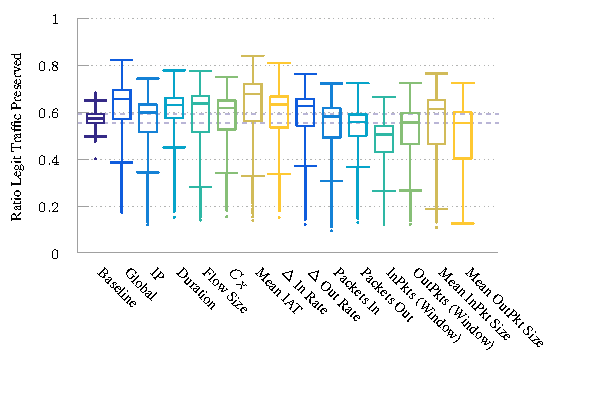
\includegraphics[width=0.8\linewidth]{../plots/ftprep-cap-box}
	\vspace{-1cm}
	\caption{
		Learned performance of Instant Control agents when benign traffic is UDP-like, using only a single feature.
%		Mean IAT, inbound packet sizes, and global state offer the best predictive performance.
		\vspace{-1em}
		\label{fig:udp-feature-plots}
	}
\end{figure}

%\begin{figure}
%	\centering
%	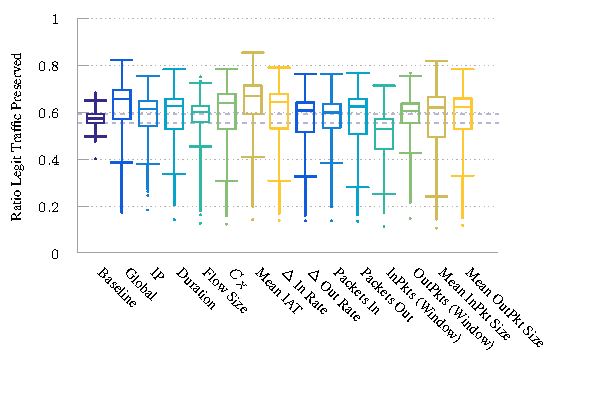
\includegraphics[width=\linewidth]{../plots/ftprep-laf-cap-box}
%	\vspace{-1.2cm}
%	\caption{
%		?? UDP, combined with last action.
%		\label{fig:udp-laf-feature-plots}
%	}
%\end{figure}

\begin{figure}
	\centering
	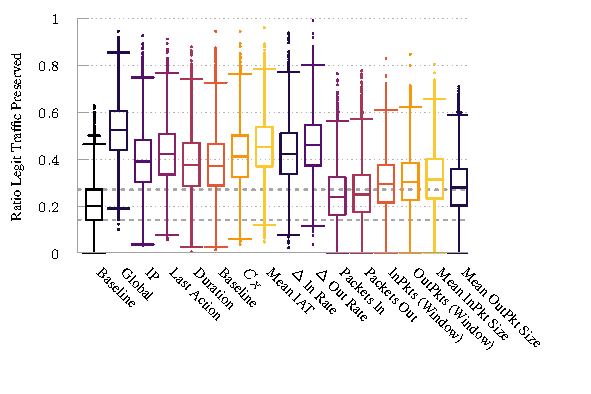
\includegraphics[width=0.8\linewidth]{../plots/ftprep-tcp-cap-box}
	\vspace{-1cm}
	\caption{
		Learned performance of Instant Control agents when benign traffic is TCP-like, using only a single feature.
%		All of the chosen features can offer a marked improvement over no protection at all.
%		Global state and Mean IAT still offer the greatest improvement above baseline.
		\vspace{-1em}
		\label{fig:tcp-cap-feature-plots}
	}
\end{figure}

\begin{table}
	\centering
	\caption{Tile coding windows for each feature.\label{tab:codings}}
	
	\resizebox{0.45\linewidth}{!}{
		\begin{tabular}{@{}ll@{}}
			\toprule
			New Feature (unit) & Range \\
			\midrule
			Load (\si{\mega\bit\per\second}) & $[0, U_s]$ \\
			IP & $[0, 2^{32}-1]$ \\
			Last Action (\si{\percent}) & $[0, 1]$ \\
			Duration (\si{\milli\second}) & $[0, \num{2000}]$ \\
			Size (\si{\mebi\byte}) & $[0,10]$ \\
			Correspondence Ratio & $[0,1]$ \\
			Mean IAT (\si{\milli\second}) & $[0, \num{10000}]$ \\
			$\Delta$In/Out Rate (\si{\mega\bit\per\second}) & $[-50, 50]$ \\
			Packets In/Out & $[0, 7000]$ \\
			Packets In/Out Window & $[0, 2000]$ \\
			Mean In/Out Packet Size (\si{\byte}) & $[0, 1560]$ \\
			\bottomrule
		\end{tabular}
	}
	\vspace{-1em}
\end{table}


%\begin{figure}
%	\centering
%	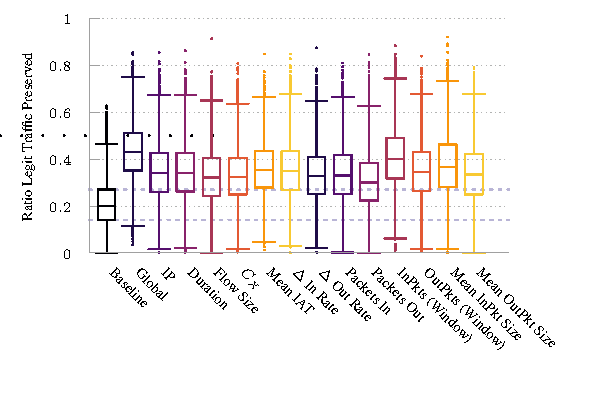
\includegraphics[width=0.8\linewidth]{../plots/ftprep-tcp-laf-cap-box}
%	\vspace{-1cm}
%	\caption{
%		Learned performance of Instant Control agents when benign traffic is TCP-like, combining each feature with the last action taken.
%		\label{fig:tcp-laf-feature-plots}
%	}
%\end{figure}

%\section{Rethinking the State Space}\label{sec:rethinking-the-state-space}
%
%Per-flow agents require features which offer high predictive power, making behavioural differences readily apparent.
%Expanding on the measures discussed in \cref{sec:motivation}, we believe the following features to be useful (and humanly justifiable), and investigate their use on different traffic types:
%%?? We use these features, and why...
%
%\fakepara{Global state}
%This is the vector of current load measurements along a flow's path introduced in \cref{sec:feature-space}.
%These values indicate the overall health of the network, and crucially are all measurements which an agent directly controls.
%
%\fakepara{Source IP address}
%Ordinarily trivial to spoof, though reflectors are themselves legitimate services being abused by spoofing attackers.
%As a result, they communicate with attack victims using their own IP address.
%In real-world scenarios the addresses of a set of reflector nodes might exhibit CIDR block similarity \cite{DBLP:conf/imc/CollinsSFJWSK07}, e.g., similarly unhardened services exposed by a single organisation.
%
%\fakepara{Last action taken}
%An agent's current belief in the maliciousness of a flow.
%This feature also serves as a reference point for determining whether a flow is actually malicious based on its response.
%This feature only makes sense when combined with another flow feature, and never appears individually tile-coded.
%
%\fakepara{Flow duration and size}
%Features which describe the length of time a connection has been active, and the amount of data transferred within that time.
%An extraordinarily long flow, having sent a lot of data, could be more likely to be an amplifier: though most (\SI{62}{\percent}) waves of amplifier traffic last shorter than \SI{15}{\minute} \cite{DBLP:conf/raid/KramerKMNKYR15}, this is considerably longer than the typical length of an HTTP request/response.
%
%\fakepara{Correspondence ratio}
%The ratio between upstream and downstream traffic for a source IP.
%We define this to be $C_X = \min(\uload{\cdot}, \dload{\cdot})/\max(\uload{\cdot}, \dload{\cdot})$, where a value close to 0 indicates strong asymmetry.
%
%\fakepara{$\mathbf{\Delta}$ Send/receive rate}
%The change in traffic rates caused by the last action.
%Behavioural changes induced by bandwidth expansion/reduction are expected to be most visible in these fields.
%
%\fakepara{Mean inter-arrival time (IAT)}
%A measure of how often packets arrive at the agent's parent switch; low IATs indicate a high number of packets per second, and can be a possible marker of malicious behaviour.
%We only make use of the mean IAT of \emph{inbound} traffic.
%
%\fakepara{(Per-window) packet count}
%The amount of packets sent to/from a source over a flow's lifetime (or the current window of measurement), similar in use to flow size and mean IAT.
%
%\fakepara{Mean packet size per window}
%Legitimate flows, both TCP- and UDP-based, often transmit packets with a distribution of sizes.
%Attack traffic is not likely to be so diverse: we might expect solely max-size packets in the case of amplification attacks, or minimum-size packets in other classes of flooding attack.
%
%The exclusion of features such as source/destination ports or protocol numbers is a deliberate choice.
%If \emph{QUIC} (or a similar protocol) were to become ubiquitous, then these fields would have no correlation with the class of traffic a flow contains.
%
%All of the above features, save for global state, are 1-dimensional.
%\Cref{fig:udp-feature-plots} shows the effectiveness of each feature for UDP (resp.\ \cref{fig:tcp-cap-feature-plots} for TCP), using a single-destination topology (\cref{sec:single-dest}) with $n=2$ hosts per egress point averaged over 10 episodes.
%%\Cref{fig:tcp-laf-feature-plots} demonstrates how feature accuracy varies when tiled alongside \emph{last action}, with similar trends being observed when the same technique is applied with UDP traffic (omitted).
%%?? Core findings---different protocols need different features, so everything we proposed above has a use!
%The plots demonstrate that different protocols and traffic classes are best defended by different features---as such, every feature presented has value in a complete model.
%Packet-level and per-window statistics are at their based when combined with the last action for both UDP-like and TCP-like traffic (omitted).
%All features converge to their highest-observed performance within around \num{4000} timesteps.
%In general, some of the most effective features are the global state, mean IAT, mean inbound packet size and $\Delta$ rates.
%?? How do they do when combined after individual training? Pretty well, especially for TCP.
%Additional testing shows that the learned per-feature policies may be easily combined (by summing action values), and that this technique is particularly effective for TCP; these results are omitted to preserve space.
%In no cases, however, do we manage to completely block attack traffic---at convergence, we observe that system load remains consistently at $U_s$.

\section{A New Normal}\label{sec:a-new-normal}

%In establishing...
%
%?? How will I structure this?
%?? Motivation -> Model -> Results?
%?? OR Use the results of the last section to springboard into here?

%From what we have seen, it is difficult (or impossible) for trace-based or numerical simulations to correctly capture certain dynamics without an extraordinary amount of care or consideration.
%As it turns out, 
%Our goal is to briefly describe an environment which tests \emph{specific} behaviours to examine the \emph{specific} problems which have arisen during our testing of past approaches.
Our network model allows live testing of reactive TCP and UDP traffic in an SDN environment, over arbitrary topologies, with an explicit focus on preserving real-time dynamics in a way that trace-based evaluation cannot.
We are primarily interested in load and packet inter-arrival characteristics, and in how they evolve in response to agent actions.
%We aim to capture interactive, correlated back-and-forth exchanges associated with live traffic.
%Naturally, this model is not perfect or representative for all traffic, yet it captures some of the behaviour which we expect will plague most legitimate TCP flows.
%If need be, we expect the frequency or distribution of requests could be conditioned to match observations of real-world access patterns.

%?? ANGLE: set up an environment to test \emph{specific} behaviours to examine \emph{specific} problems in past work. I make no claims that it is perfect or representative for all traffic, just for this (likely common) behaviour which I expect to plague almost all legit TCP flows.

%?? Existing sims used for testing such applications reliant on traces, or not sophisticated enough to capture interactive, back-and-forth (correlated) behaviours---possibly discarded as second-hand effects by past work when these are so crucial given user traffic patterns (and the nature of the control signal we choose to enact).

%?? Remember, the motivation is clear. We don't care so much that it is "representative" wrt a specific deployment location or network type. The whole purpose of this is that we aim to test specific behaviour which traces cannot replicate (i.e., correlated back-and-forth, dynamics introduced to congestion-aware protocols, ...)
%?? If we need to, we can condition the distribution of requests according to statistics mined from an existing trace if reviewer number 2 needs that extra push to be convinced.

\subsection{Network Design}
We make use of a fully software-defined network, built using OpenFlow-aware switches in mininet alongside a controller application based on \emph{Ryu} \cite{ryu}.
Internal routers begin with knowledge of the shortest path to each protected host, while inbound flows register their return path at each hop, ensuring consistent traffic conditions for each flow.
OpenFlow \emph{group actions} provide consistent multipath routing where needed. 
%If several ports offer different (equal-length) paths to a destination, a consistent random port is chosen from the flow-hash by an OpenFlow \emph{Group action} (in \emph{select} mode).
%If such information is lost, perhaps expiring due to inactivity, it suffices to forward an outbound packet on a random (outbound) port, as we assume that any external IP is reachable through any of the test network's egress ports (i.e., that it is not connected to any stub autonomous systems).
The controller is also responsible for computing how switches respond to ARP requests: this need arises due to the reliance upon Linux's networking stack for live applications.
%We make further use of the topology presented earlier (\cref{sec:topology}), noting that our architecture allows us to trivially extend and modify this if required.

\subsection{TCP (HTTP) Traffic Model}
%?? Legitimate traffic: TCP traffic (HTTP clients downloading web pages, dependent resources and files) with a mixture of lifetimes for each request.
To model legitimate TCP traffic, server nodes run an nginx v1.10.3 HTTP daemon, serving statically generated web pages alongside various large files and binaries.
Benign hosts repeatedly request resources from the server via libcurl.
Both use the TCP Cubic \cite{rfc8312} flavour of TCP.
A host's download rate is limited to match its assigned maximum bandwidth, and requests several files known to exist within a website, followed by dependencies for each (stylesheets, images, etc.).
This presents a balanced distribution of flow duration and size, with large files included to model bulk transfer.
On completion, a host changes its IP to generate separate statistics per flow.

\subsection{UDP (Opus) Traffic Model}
VoIP traffic is heavily different to the above model; packet arrivals are highly periodic due to real-time requirements, flows are constant bitrate, and do not react substantially to lost packets.
DDoS attack traffic is known to share many of these characteristics, offering an interesting detection problem.
We present a traffic model\footnote{Repository link removed for double-blind reviewing.} based on Discord\footnote{\url{https://discord.gg}}, a messaging and VoIP platform.
%We present a VoIP traffic model\footnote{\url{https://github.com/FelixMcFelix/opus-voip-traffic}} based on Discord\footnote{\url{https://discord.gg}}, a freely-available messaging and VoIP platform geared toward video game communities.
We use this as our prototype due to its public API, open source frameworks, and the lack of models for Opus-encoded traffic.
All parameters (save for truncating silent periods) are derived from passive measurement, API documentation, and community observations.
%?? Highly periodic, CBR

Discord hosts send RTP traffic with Salsa20 encrypted payloads---audio frames of length \SI{20}{\milli\second} at a target \SI{96}{\kilo\bit\per\second}.
Hosts generate similar traffic by replaying anonymised traces; each contains the size of an audio payload, missed packets, and silent durations.
We trim silent periods to a maximum \SI{5}{\second} due to lengthy talk/silence bursts of users in RPG servers, and estimate the size of missed packets with an exponentially-weighted moving average.
Hosts transmit a 4-byte keepalive every \SI{5}{\second}.
A central server groups hosts into rooms, and forwards packets to other participants; we do not replicate pre-call Websocket traffic which would be used for authentication.
There is no peer-to-peer traffic---the server acts as a TURN relay for all hosts.
%?? Reflective factor among \emph{authenticated hosts}.
We find that each flow occupies an expected \SI{52.4}{\kilo\bit\per\second} upstream bandwidth.
To match the target upload rate assigned to each host, it runs enough individual sessions to meet the target data rate.

%?? Malicious traffic: UDP flood traffic (hping3, MTU-size packets, ). Why not min-size packets? Because the traffic generator gets in a horrible rut if I do so...

\section{Evaluation}

%Traffic is played back from hosts via Tcpreplay at a bandwidth assigned uniformly from a `good' or `bad' distribution, each using the same pcap file with source and destination IP addresses rewritten.

We compare our work's performance and learning rate against Marl \cite{DBLP:journals/eaai/MalialisK15}, the state-of-the-art in RL-based DDoS prevention, across different topologies and workloads.
We made use of the OPUS and TCP traffic models introduced in \cref{sec:a-new-normal}, both topologies discussed below (1-dest vs Fat-Tree), and varied the amount of hosts communicating over each egress node.
Additionally, we evaluated these models in multi-agent (\emph{separate}, no model sharing) and single-agent modes (\emph{single}, 0-cost perfect information sharing).
In each case, the algorithm's performance was averaged over \num{10} episodes of length \num{10000} timesteps (resetting policies between episodes).
Host allocations at the beginning of each episode were generated pseudorandomly to ensure fairness between episodes.
Malicious traffic is provided by \emph{hping3}, generating UDP-flood traffic targeting random ports with MTU-sized packets.
All experiments were executed on Ubuntu 18.04.2 LTS (GNU/Linux 4.4.3-040403-generic x86\_64), using a 4-core Intel Core i7-6700K (clocked at \SI{4.2}{\giga\hertz}) and \SI{32}{\gibi\byte} of RAM.
%All code underpinning these findings is available on a public repository\footnote{\url{https://github.com/FelixMcFelix/rln-dc-ddos-paper}}.
%All code underpinning these findings is available on a public repository.\footnote{Private until publication.}

\subsection{Single Destination}\label{sec:single-dest}
The network is tree-structured: one server $s$ connects through a dedicated switch to $k$ team leader switches, each connected to $\ell$ intermediate switches, which in turn each connect to $m$ egress switches.
$n$ hosts then connect through each egress switch.
We thus have $N_{\mathit{hosts}} = k \ell m n$.
We configured the network topology using $k=2$ teams, $\ell=3$ intermediate nodes per team, $m=2$ agents per intermediate node, and $n \in \{2, 4, 8, 16\}$ hosts per learner.
This is a slight simplification of the \textquote{online} experiment of \textcite{DBLP:journals/eaai/MalialisK15}, choosing fewer teams but similar structure.

%\begin{figure}
%	\centering
%	\resizebox{0.8\linewidth}{!}{
%		\begin{tikzpicture}[
%		texts/.style = {text=black},
%		labeltexts/.style = {text=uofgsandstone},
%		treeline/.style = {draw=uofgburgundy},
%		treenode/.style = {texts, circle, centered, fill=white, treeline},
%		load/.style = {fill=uofgcobalt},
%		loadhide/.style = {fill=uofgcobalt!40!white},
%		external/.style = {fill=uofgrust},
%		externalhide/.style = {fill=uofgrust!40!white},
%		hideline/.style = {draw=uofgsandstone!40!white},
%		hidenode/.style = {treenode, hideline},
%		grow'=right
%		]
%		\node[treenode, label={[texts]above:Server}] (root) {}
%		child [treeline] { node [treenode, label={[texts]above:Core}] (sswitch) {}
%			child [treeline] { node [treenode, label={[texts]above:Leader}] (teaml) {} 
%				child [treeline] { node [treenode, label={[texts]above:Intermediate}] (inter) {}
%					child [treeline] { node [treenode, load, label={[texts]above:Agent/Egress}] (agent) {}
%						child [treeline] { node [treenode, external] (extern) {}
%							child [treeline] { node [treenode, external, label={[texts]above:Host}] (host) {} }
%							child [hideline] { node [hidenode, externalhide] (endhost) {} }
%						}
%					}
%					child [hideline] { node [hidenode, loadhide] (endagent) {} }
%				}
%				child [hideline] { node [hidenode] (endinter) {} }
%			}
%			child [hideline] { node [hidenode] (endteaml) {} }
%			edge from parent
%			node[below, labeltexts] {$U_s$}
%		};
%		
%		%\draw[-] (teaml) -- (endteaml);
%		\node [labeltexts] (kdots) at ($(teaml)!0.5!(endteaml)$) {$\rvdots$};
%		\node [labeltexts, right = -0.1cm of kdots] {$k$};
%		\node [labeltexts] (ldots) at ($(inter)!0.5!(endinter)$) {$\rvdots$};
%		\node [labeltexts, right = -0.1cm of ldots] {$\ell$};
%		\node [labeltexts] (mdots) at ($(agent)!0.5!(endagent)$) {$\rvdots$};
%		\node [labeltexts, right = -0.1cm of mdots] {$m$};
%		\node [labeltexts] (ndots) at ($(host)!0.5!(endhost)$) {$\rvdots$};
%		\node [labeltexts, right = -0.1cm of ndots] {$n$};
%		\end{tikzpicture}
%	}
%	\caption{
%		Network topology diagram, showing how the server and its core switch's $k$ teams are structured, with $\ell$ intermediate routers per team, connected to $m$ agents which each moderate $n$ hosts beyond a single external switch.
%		%	Empty nodes are considered to be internal.
%		Red nodes are external, and each blue node hosts an agent.
%		\vspace{-1em}
%		\label{fig:marl-topol}
%	}
%\end{figure}

\subsection{Multiple Destinations}
The previous topology allows for direct comparison against the state-of-the-art, however it is hard to argue its relevance to specific classes of victim or how it might interact with applications.
In contrast, the fat-tree topology \cite{DBLP:conf/sigcomm/Al-FaresLV08} sees regular use in real-world datacentres and scales well horizontally.
We use a $k=4$ fat-tree, with one pod hosting two servers $s_0$ and $s_1$.
$n$ external hosts connect through each core switch (where agents are hosted), and communicate with $s_0, s_1$ uniformly randomly.
Both servers host identical services.
We set $n \in \{6, 12, 24, 48\}$ hosts per learner (keeping $N_{\mathit{hosts}}$ identical to each tier of the single-host topology), and restrict $U_{s_0} = U_{s_1} = U_s / 2$.

\subsection{Parameters}
Algorithm parameters were set at $\alpha=0.05$, linearly annealing $\epsilon=0.2 \rightarrow 0$ by $t=3000$ in the case of Marl (\num{8000} actions per agent in the \emph{Instant/Guarded} models).
Benign hosts uploaded between \SIrange{0}{1}{\mega\bit\per\second}, and hosts were redrawn each episode with $\operatorname{P}(\mathit{malicious})=0.4$.
Malicious hosts sent \SIrange{2.5}{6}{\mega\bit\per\second} when attacking UDP traffic, increased to \SIrange{4}{7}{\mega\bit\per\second} for TCP-like or mixed traffic to meaningfully impact benign flows.
Given $n$ and $\operatorname{P}(\mathit{malicious})$, we see an expected malicious bandwidth \numrange{1.27}{1.87} and \SIrange{2.03}{2.18}{$\! \times U_s$} respectively.
$U_s$ was fixed at $N_{\mathit{hosts}}+2$ \si{\mega\bit\per\second} (to account for burstiness), and each link had a delay of \SI{10}{\milli\second}.
All links had unbounded capacity, save for server-switch connections.
These parameter choices match those of the original study for direct comparison, but we justify our range of $n$ as capturing increasing scales of host activity.

\section{Results and Discussion}
\label{sec:the-results-of-doing-so}

We now compare the performance of our two new models (\emph{Instant}, \emph{Guarded}) against existing RL work (\emph{Marl}) with different traffic and topologies, varying the host-to-learner ratio $n$.
%?? Probably best just to look at top level stuff, and THEN a simplified comparison for each intended improvement (like banded rewards).
%Additionally, we examine the performance effects of environmental characteristics and potential improvements: negative reinforcement, the case where one agent makes all decisions, and pre-training on individual features.
We present the average rewards for all combinations of these factors in \crefrange{tab:av-vals}{tab:av-ecmp-vals}---providing a rough idea of expected performance, with the highest-performing model in bold.
We include plots which paint a different picture, showing peak performance and the amount of time an agent needs to learn.

\begin{table}
	\centering
	\caption{Average reward for combinations of model, host density and traffic class with a single destination.\label{tab:av-vals}}
	
	\resizebox{0.8\linewidth}{!}{
		\expandableinput ../tables/infocom-tree-avg-reward.tex
	}
\vspace{-1em}
\end{table}
\begin{table}
	\centering
	\caption{Average reward for combinations of model, host density and traffic class with multiple destinations.\label{tab:av-ecmp-vals}}
	
	\resizebox{0.8\linewidth}{!}{
		\expandableinput ../tables/infocom-ecmp-avg-reward.tex
	}
\vspace{-1em}
\end{table}

\subsection{Congestion-unaware traffic}
%\begin{figure}
%	\centering
%	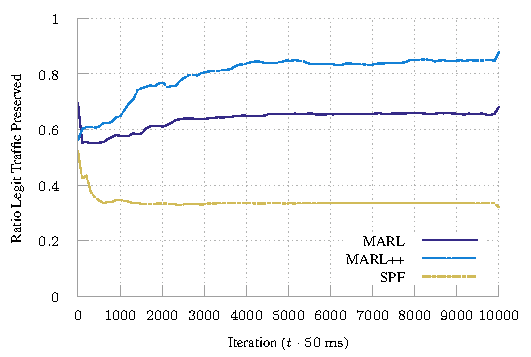
\includegraphics[width=0.9\linewidth]{../plots/udp-2}
%	
%	\caption{
%		Online performance for $n=2$ hosts per egress point when benign traffic is UDP-like.
%		Although Marl++ offers a marked improvement (a peak $\sim$\SI{30}{\percent} more benign traffic arrives unimpeded), SPF significantly underperforms for this relatively simple topology.
%		Non-SPF agents start off reasonably well, slowly learning better policies.
%		\label{fig:udp-2}
%	}
%\end{figure}
%\begin{figure}
%	\centering
%	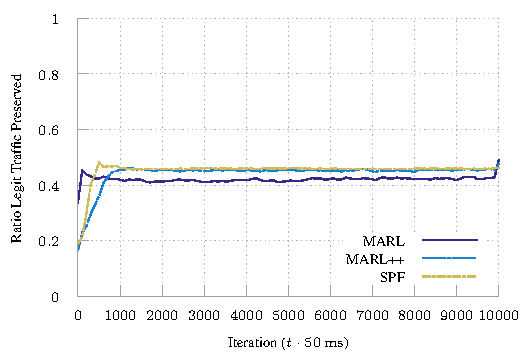
\includegraphics[width=0.9\linewidth]{../plots/udp-16}
%	
%	\caption{
%		Online performance for $n=16$ hosts per egress point when benign traffic is UDP-like.
%		Marl++ remains marginally ahead of its predecessor, though both have undergone a significant drop in effectiveness.
%		SPF, remarkably, displays performance on par with Marl++ for this more difficult topology.
%		Both of the new models take longer to train, but achieve better peak and average performance than Marl.
%		\label{fig:udp-16}
%	}
%\end{figure}
\begin{figure}
	\centering
	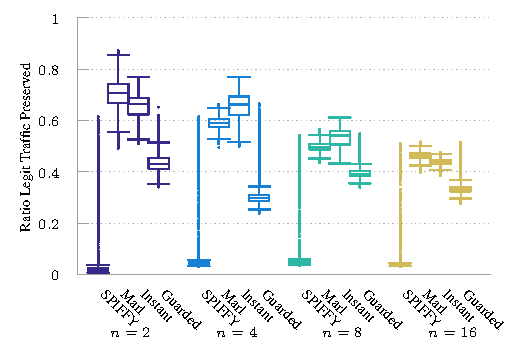
\includegraphics[width=0.75\linewidth]{../plots/tnsm-udp-box-separate}
	\vspace{-1em}
	\caption{
		Online performance for Opus benign traffic in a single-destination network, multi-agent mode.
%		Marl++ offers a marked improvement (a peak $\sim$\SI{30}{\percent} more benign traffic arrives unimpeded) at small $n$, and remains marginally ahead of its predecessor by $n=16$, though both have undergone a significant drop in effectiveness.
%		\emph{Instant} outperforms Marl for $n \in \{4, 8\}$ (with higher variance), but performs similarly to Marl at $n\in \{2, 16\}$.
		\emph{Guarded} always underperforms.
%		SPF, remarkably, slightly outperforms Marl++ (with lower variance) for this more difficult topology despite being worse for smaller $n$.
%		Both of the new models take longer to train, but achieve better peak and average performance than Marl.
%		?? REWORK/MAKE ACCURATE
		\vspace{-1em}
		\label{fig:udp-tree-box}
	}
\end{figure}

%\begin{figure}
%	\centering
%	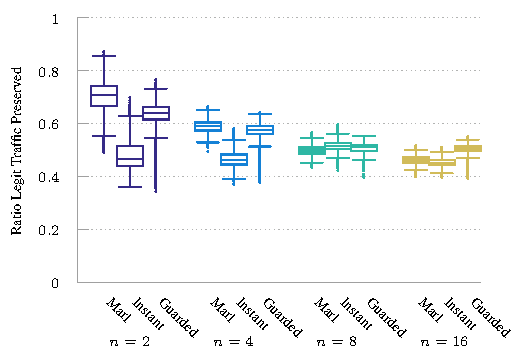
\includegraphics[width=0.95\linewidth]{../plots/tnsm-udp-box-single}
%	
%	\caption{
%		Online performance for Opus benign traffic in a single-destination network, single-agent mode.
%		?? DO I need this?
%		\label{fig:udp-tree-box-single}
%	}
%\end{figure}
%
%\begin{figure}
%	\centering
%	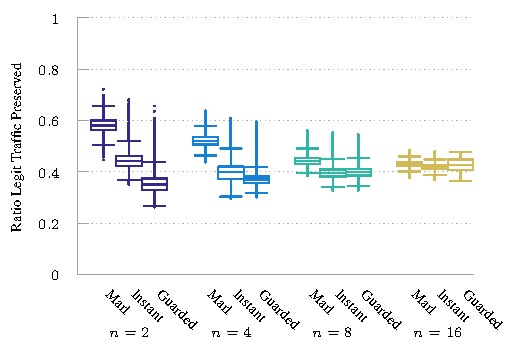
\includegraphics[width=0.95\linewidth]{../plots/tnsm-ecmp-udp-box-separate}
%	
%	\caption{
%		Online performance for Opus benign traffic in a multi-destination network, multi-agent mode.
%		?? DO I need this?
%		\label{fig:udp-ecmp-box}
%	}
%\end{figure}
%
%\begin{figure}
%	\centering
%	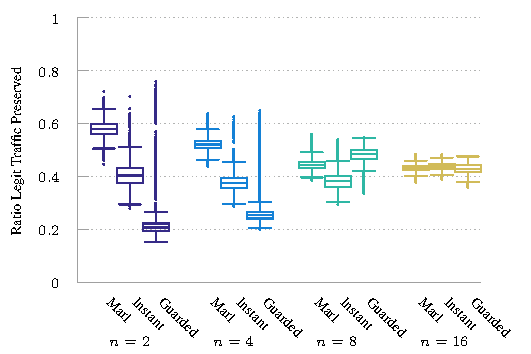
\includegraphics[width=0.95\linewidth]{../plots/tnsm-ecmp-udp-box-single}
%	
%	\caption{
%		Online performance for Opus benign traffic in a multi-destination network, single-agent mode.
%		?? DO I need this?
%		\label{fig:udp-ecmp-box-single}
%	}
%\end{figure}

In a single-destination network, we observe that Marl's performance degrades as $n$ increases.
Typically, \emph{Instant} agents achieve the best performance in multi-agent mode, reducing collateral damage above the current state-of-the-art, but sharply degrade at low $n$ when agents share experience.
We see a reversal of this trend for the \emph{Guarded} model, which improves as $n$ increases and in single-agent mode---when $n\ge4$, the single-agent variant offers consistent improvement.
%Across all choices of $n$, we see that Marl++ exhibits reduced collateral damage compared to Marl, with SPF starting poorly yet becoming more effective for larger $n$ (\cref{tab:av-vals}, \emph{Capped}, UDP).
\Cref{fig:udp-tree-box} shows the preserved traffic in multi-agent mode.
%?? Discuss multi-dest topol once all results available.
When defending multiple destinations, we see a sharp decrease in the effectiveness of all agent designs.
\emph{Instant} and \emph{Guarded} agents become more effective as $n$ increases, while Marl's effectiveness is roughly constant (aside from the outlier at $n=12$).

%Although we improve upon Marl in both identified problem cases, the improvements are small for UDP traffic.
The most likely explanation for low UDP protection is that agents are converging to, and becoming stuck in, locally optimal (but globally sub-optimal) policies.
The increased state space size and similar characteristics between benign and attack traffic make this more likely.
These difficulties may be further worsened by the competitive nature of multi-agent learning.
Paradoxically, \emph{Instant} actively suffers when trained as a single learner---this may occur due to even spreads of values between widely different actions, due to shared characteristics between legitimate and malicious flows.

\subsection{Congestion-aware traffic}
%\begin{figure}
%	\centering
%	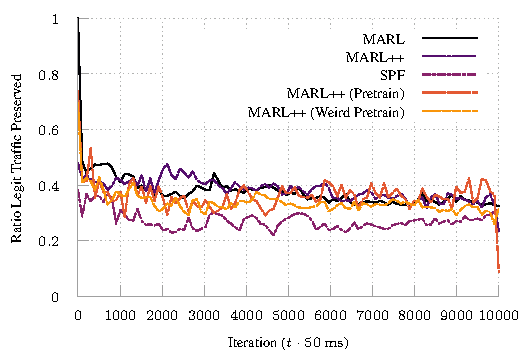
\includegraphics[width=0.9\linewidth]{../plots/tcp-2}
%	
%	\caption{
%		Online performance for $n=2$ hosts per egress point when benign traffic is TCP-like.
%		Marl++ and Marl achieve very similar performance, starting off similarly well without notable improvement over an episode.
%		SPF's performance is disappointingly close to baseline, indicating that it is as useful as having no defence system.
%		\label{fig:tcp-2}
%	}
%\end{figure}
\begin{figure}
	\centering
	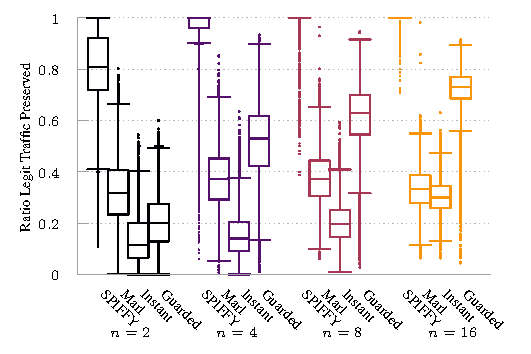
\includegraphics[width=0.75\linewidth]{../plots/tnsm-tcp-box-single}
	\vspace{-1em}
	\caption{
		Online performance for HTTP benign traffic in a single-destination network, single-agent mode.
%		\emph{Instant} and \emph{Guarded} exhibit essentially identical efficacy at $n~=~2$, protecting less traffic than Marl.
%		Longer tails of outliers typically indicate longer training.
%		\emph{Guarded}'s performance rapidly increases with $n$, achieving considerably better median performance and lower variance than the other models.
%		Longer tails of outliers typically indicate longer training times---we observe that \emph{Guarded} has considerably lower variance once it has converged on a stable policy.
		\label{fig:tcp-tree-box}
	}
\vspace{-1em}
\end{figure}
%\begin{figure}
%	\centering
%	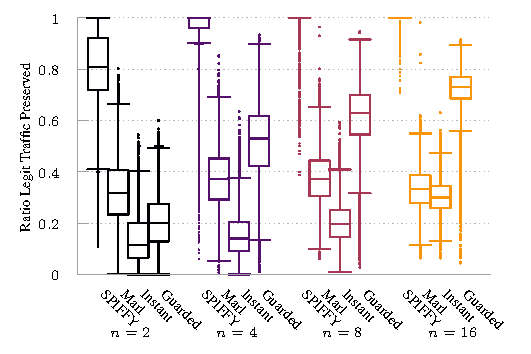
\includegraphics[width=0.95\linewidth]{../plots/tnsm-tcp-box-single}
%	
%	\caption{
%		Online performance for HTTP benign traffic in a single-destination network, single-agent mode.
%		?? DO I need this?
%		\label{fig-tcp-tree-box-single}
%	}
%\end{figure}
\begin{figure}
	\centering
	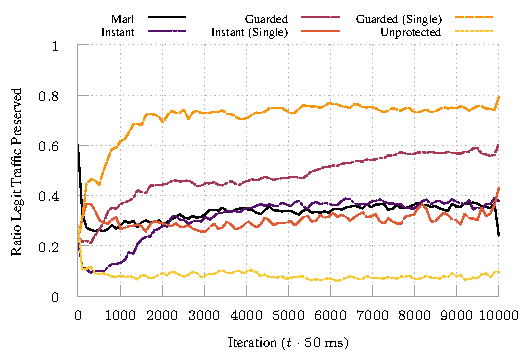
\includegraphics[width=0.75\linewidth]{../plots/infocom-tcp-16-single}
	\vspace{-1em}
	\caption{
		Online performance of standard and single-agent models over time (TCP, $n=16$, tree).
%		At this level of host density, \emph{Guarded} reaches higher peak performance sooner and is considerably more consistent throughout the episode.
%		\emph{Guarded} benefits greatly from information sharing, converging to protect around \SI{75}{\percent} of TCP traffic within \SI{100}{\second}.
%		The \emph{Instant} model converges to Marl's level of performance.
%		With a single agent, Marl++ shows worse performance, while SPF improves significantly and continues to learn well past annealing $\epsilon \rightarrow 0$.
		\label{fig:tcp-tree-16}
	}
\vspace{-1em}
\end{figure}

%\begin{figure}
%	\centering
%	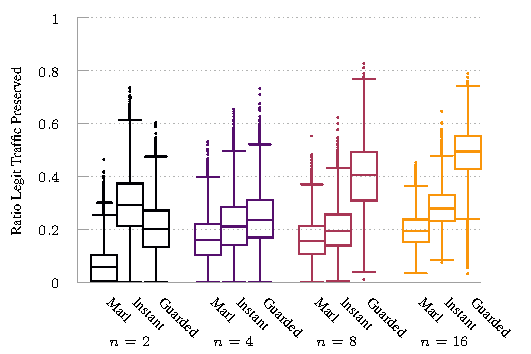
\includegraphics[width=0.95\linewidth]{../plots/tnsm-ecmp-tcp-box-separate}
%	
%	\caption{
%		Online performance for HTTP benign traffic in a multi-destination network, multi-agent mode.
%		?? DO I need this?
%		\label{fig:tcp-ecmp-box}
%	}
%\end{figure}

%\begin{figure}
%	\centering
%	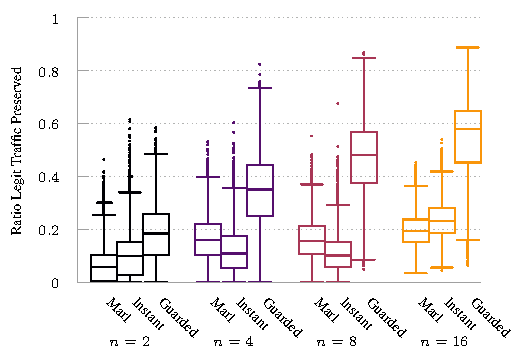
\includegraphics[width=0.95\linewidth]{../plots/tnsm-ecmp-tcp-box-single}
%	
%	\caption{
%		Online performance for HTTP benign traffic in a multi-destination network, single-agent mode.
%		?? DO I need this?
%		\label{fig:tcp-ecmp-box-single}
%	}
%\end{figure}

%\begin{figure}
%	\centering
%	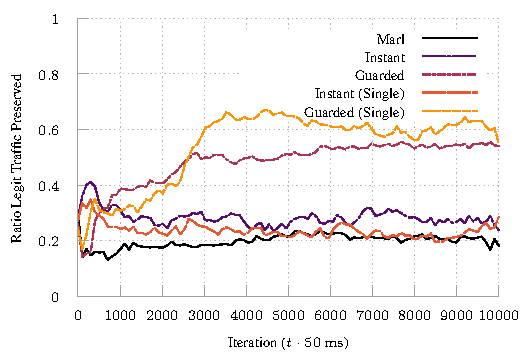
\includegraphics[width=0.95\linewidth]{../plots/tnsm-ecmp-tcp-16-single}
%	
%	\caption{
%		?? Eh
%		\label{fig:tcp-ecmp-16}
%	}
%\end{figure}

\Cref{tab:av-vals} shows that Marl offers a low level of protection for TCP traffic, which the \emph{Instant} agent offers little improvement over.
However, \emph{Guarded} agents fare substantially better, particularly when experience can be shared---offering a \SI{2.21}{$\!\times$} improvement over the state-of-the art during training, which is made clearer in \cref{fig:tcp-tree-box}.
\Cref{fig:tcp-tree-16} shows that this model can protect a peak \SI{80}{\percent} of TCP traffic (\SI{2.5}{$\!\times$} improvement over Marl, \SI{8}{$\!\times$} more traffic than no defence system) after just \SI{100}{\second}, but also that all of the new models require considerably longer than Marl to learn their best-achieving policy.
%SPF reaches a stronger plateau before \emph{both}, remaining more consistent and appearing to continue learning.
%?? Discuss multi-dest topol once results available.
The same trends are present in the multi-destination topology: \emph{Guarded} remains the best fit for TCP, in both training modes.
Crucially, the rigid tree of learners and teams which define Marl, along with its lack of action granularity, seem to be a poor fit in this environment.

\emph{Guarded}'s unpredictable and worse starting performance is unexpected, given its smaller action space.
We expected that this would make the model easier to learn, but the extra state required appears to make the task initially \emph{harder}.
This design performs best (with considerably lower variance) when agents gain as much experience as possible: high $n$ and single-agent training.
To filter traffic, it must degrade a flow multiple times in a row, reducing the likelihood that a legitimate flow is punished by accident.
We claim \emph{Guarded} is a stronger model for these reasons, and its successes offer strong rationale to consider the best schemes for efficient information sharing.

%\subsection{Single-agent performance}
%Making all decisions with a single agent is roughly equivalent to having a zero-cost communication channel between each pair of agents, theoretically allowing faster training by giving each agent more experience.
%Curiously, we observe that this often leads to drastically worse policies when used as part of Marl++ for small $n$, but makes SPF a considerably more competitive model---especially for TCP, and as $n$ grows larger (\cref{fig:tcp-16}).
%Single-agent SPF almost consistently outperforms Marl.
%We discuss our conjectures for why this reversal occurs in \cref{sec:discussion}.

%\subsection{Computational Cost}
%%?? Consider talking about the execution times of the old MARL approach here? They're real nice (as expected), so we have lots of room to play around with while (hopefully) remaining under the 1ms target time given by \textcite{DBLP:conf/sigcomm/ChenL0L18}.
%
%%Overall, each episode takes around \SI{10}{\minute} to run, while each set of \num{10} requires around \SI{2}{\hour} due to additional set-up/tear-down costs associated with mininet.
%Measurements taken during each of these experiments indicated that the cost of computing any action is typically within \SIrange{80}{100}{\micro\second}.
%This is reassuring when measured alongside the insights from other work, since as we discussed in \cref{sec:systems-considerations} the python language bottlenecks performance.
%\Textcite{DBLP:conf/sigcomm/ChenL0L18} observe that, ideally, actions must be computed and taken within \SI{1}{\milli\second} to have a meaningful affect on short flows.
%%Most flows are short, and flow-size follows a heavy-tailed distribution.
%That our starting point falls significantly below this threshold allows us to safely consider more costly actions or larger state spaces, which would typically increase the computational cost.
%?? TODO: update with modern numbers...

\subsection{RL algorithms}
When choosing a learning algorithm, we compared semi-gradient Sarsa against Q-learning, and variants of these algorithms based on \emph{eligibility traces} (Sarsa($\lambda$), Watkins's Q($\lambda$)).
Our experiments found that Sarsa offered the best performance and behaviour; \cref{fig:algo-spf-tcp} shows a trend observed across model choices and communication except for multiagent \emph{Instant} protection of TCP where Q-learning succeeds.

\begin{figure}
	\centering
	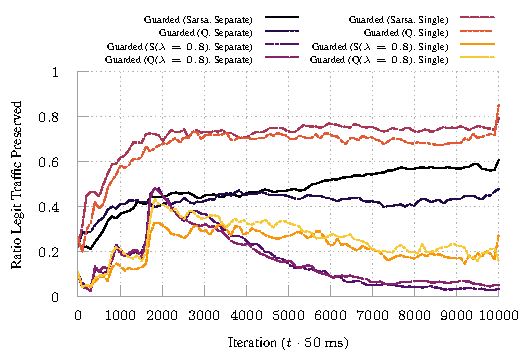
\includegraphics[width=0.75\linewidth]{../plots/tnsm-algo-spf-tcp}
	\vspace{-1em}
	\caption{
		Comparison of RL algorithms for \emph{Guarded} (TCP, $n=16$, tree).
		%		At this level of host density, \emph{Guarded} reaches higher peak performance sooner and is considerably more consistent throughout the episode.
		%		\emph{Guarded} benefits greatly from information sharing, converging to protect around \SI{75}{\percent} of TCP traffic within \SI{100}{\second}.
		%		The \emph{Instant} model converges to Marl's level of performance.
		%		With a single agent, Marl++ shows worse performance, while SPF improves significantly and continues to learn well past annealing $\epsilon \rightarrow 0$.
		\label{fig:algo-spf-tcp}
	}
\vspace{-1em}
\end{figure}

\section{Related Work}\label{sec:related-work}

%?? Try and compare my work here when possible?

\fakepara{DDoS Prevention}
\Textcite{DBLP:conf/lcn/BragaMP10} have examined the detection of volume-based DDoS attacks through \emph{self-organising maps}, making use of SDN to gather statistics effectively.
Many of their features aren't relevant to our work, as their focus is not active defence or discovering \emph{which} hosts are contributing to an attack.

%?? Actually talk about Marl (???) to appease reviewer \#1.
The closest approach in this field is that of \textcite{DBLP:journals/eaai/MalialisK15}, whom we have positioned our work against.
They create a tree overlay topology subdivided into teams, where each agent applies packet drop to \emph{all} inbound traffic.
%?? Recap their flaws, since they've been cut form every other aspect.
Their technique suffers at high host density and when congestion-aware traffic dominates.
%These effects are not present in their results, suggesting an evaluation driven purely by traces.

\emph{SPIFFY} \cite{DBLP:conf/ndss/KangGS16} remedies transit-link attacks by observing how flows from each source respond to a sudden increase in available bandwidth.
Bots participating in an attack cannot often match any bandwidth expansion due to having already saturated the capacity of their local outbound links.
%Attackers must either be detected or reduce the throughput of each bot, increasing the cost of launching an attack.
Unlike our approach, SPIFFY is intended to be deployed within ASes.
Its weakness is that computing a route with enough spare bandwidth can be costly, and that low expansion factors in real networks can require more rounds of testing. 
Traffic response to bandwidth expansion may not extend to HTTP DASH traffic or constant bitrate traffic (e.g., UDP VoIP traffic), which make up a sizeable portion of network traffic.

\emph{Athena} \cite{DBLP:conf/dsn/LeeKSPY17} is a general SDN framework for intrusion detection, using a \emph{k-nearest neighbours} classifier to detect individual attack flows.
Although heavyweight (and effective compared with \textcite{DBLP:conf/lcn/BragaMP10}), their comparison against SPIFFY lacks the evidence needed to draw conclusions.

\Textcite{DBLP:conf/sp/SmithS18} use AS-level routing to tackle transit-link and direct attacks.
This view is taken due to the perceived cost of per-stream classification and inherent sensitivity to adversarial examples or crafted input.
The approach uses BGP advertisements to preserve traffic to a target AS, but unlike SPIFFY the approach doesn't actually \emph{remove} the congestion.
Because of this, volume-based attacks aren't fully alleviated.

%?? Abuses of RL 
\fakepara{RL in Networks}
RL has seen little examination in the challenge of intrusion detection/prevention.
Past works use the approach as a traditional classifier \cite{shamshirband2014anomaly,DBLP:conf/mates/ServinK08}.
Given that one of the main strengths of RL techniques is the ability to control (and adapt through) ongoing interaction, these works don't apply the paradigm at its fullest potential.

Effective uses have lain in learning when it is best to \emph{communicate} and share knowledge between anomaly detectors \cite{DBLP:conf/paisi/XuSH07}, and in data-driven networking, such as for intra-AS route optimisation \cite{DBLP:conf/hotnets/ValadarskySST17} and for process allocation \cite{DBLP:conf/hotnets/MaoAMK16}.
\Textcite{DBLP:conf/sigcomm/MaoNA17} employ client-side observations of network state and video player performance to optimise adaptive bitrate selection for multimedia streaming.

\emph{AuTO} \cite{DBLP:conf/sigcomm/ChenL0L18} employs deep RL to perform traffic optimisation.
They find that the vast majority of flows are short-lived, requiring effective decisions in less than a millisecond.
To overcome the high latency of neural network computations, two agents are trained, handling aspects of short (priority thresholds) and long flows (bespoke allocations) respectively.

%These works emphasise the necessity of ingenuity in effectively handling how states and actions are represented.

\section{Conclusions and Future Work}
Through this paper, we have introduced reinforcement learning and its relevance to network intrusion prevention.
We believe that the ability to learn network control as an online feedback loop makes it particularly effective in modern networks.

We have put forth an RL agent design which acts per-flow, describing the algorithmic modifications and engineering choices needed to make its deployment feasible.
Supporting this, we've demonstrated the value of the features these agents use as evidence.
Our evaluation shows that our new agent designs considerably advance the state-of-the-art in RL-based DDoS prevention, with \emph{Guarded} agents showing the most promise for future evaluation.

The most direct improvements to be made lie in the correct protection of legitimate UDP traffic, which our agent designs have difficulty safeguarding.
Outside of this, there is scope to test these new techniques against link-flooding attacks in large-scale topologies using reward functions such as \cref{eqn:lfa-reward}.
Simulation is the most likely avenue for such evaluation.
The remaining weaknesses invite many further improvements worth investigation: the design of reward functions derived from QoE metrics, agent operation via \emph{programmable data planes} \cite{DBLP:conf/ancs/JouetP17}, and evaluation against evolving DDoS attacks \cite{DBLP:conf/spw/KangGS16}.

We hope it is clear that reinforcement learning holds promise and can inspire further innovation.
It allows us to offer distinct advantages above existing works, such as protocol-agnostic DDoS flow detection, more flexible deployment, and automatically learned low-overhead decision-making---without requiring many of the same network resources or capabilities that other techniques discussed in \cref{sec:related-work} rely upon.
Our proposed approach offers substantial improvements for the defence of congestion-aware traffic, which remains the most prevalent class of traffic on the internet today, while offering future-proofing against the introduction of new transports.
It's hoped that more research in this direction will open the door to works which capture the complex and fluid nature of modern networks; evolving topologies, traffic and protocol distributions, and attacks.

\section*{Acknowledgements}
%Our thanks go to Colin Perkins, Mircea Iordache, Qianru Zhou and Cristian Urlea for their advice, comments and technical assistance.
Our thanks go to Anonymous, Anonymous, Anonymous and Anonymous for their advice, comments and technical assistance.
%Additional thanks \emph{would} go out to my anonymous reviewers, had I any of them.
This work was supported by a nameless funder with a name approximately as long as this line [grant number 0].
%This work was supported by the Engineering and Physical Sciences Research Council [grant number EP/M508056/1].

\renewcommand*{\bibfont}{\footnotesize}
\printbibliography

\end{document}